\section{Analysing Conflict}\label{conflict}
In software development, especially in agile methods, conflict analysis is an important task to ensure the coherence and functionality of the system to be developed. A conflict is defined as a inconsistency that arises when two or more requirements, often encapsulated as USs, contradict each other. This section will introduce and define conflict analysis, focusing on the concept of \textit{content inconsistency} between USs.

The main objective of this analysis is to rationalise the software development workflow by semantically identifying conflicts between the USs within the backlog of a project.

A conflict of requirements arises when two or more USs show contradictions or inconsistencies. This can manifest itself in various forms, e.g. in the manipulation of the same resource by several USs at the same time, in overlapping functions or in conflicting conditions.

\begin{example}
	Considering following USs:\\\\
	user\_story\_13: "\#G03\# As a Staff member, I want to Apply a Hold, so that I can prevent progression through the workflow or other actions in the system until the issue is resolved."\\\\
	user\_story\_14: "\#G03\# As a Staff member, I want to Remove a Hold, so that I can allow progression through the workflow or other actions in the system now that the issue has been resolved."\\\\
	In this example, user\_story\_14 deletes a resource that is used by user\_story\_13. This means that user\_story\_13 cannot be applied at all if user\_story\_14 is executed first, which leads to a conflict between these USs.
\end{example}

In section \ref{conflict_requirement}, we present the requirements and functional needs that serve as input for the design phase in order to fulfil the requirements. In section \ref{conflict_desing} we explain the design decisions of the workflow shown in figure \ref{fig:conflict_operational_flow} and explain how the architecture is structured. 

\subsection{Requirements}\label{conflict_requirement}
In order to accomplish the analysis of conflicts in USs we try to address following functional requirements:
\begin{itemize}
	
	\item As a user, I want to perform semantic analysis on user stories within a specified project backlog, so that I can identify and address conflicts effectively.
	
	\item As a user, I want a report on the US-pairs that are conflicting in the main parts so I can change them if needed.
	
	\item As a user, I want to apply a filter to the conflict report to only show US-pairs that have the same resource (as entity) with different verbs (as action), so that the verbs are semantically contradictory (e.g. one US deletes a resource that another US is using, or deleting or one US creates a resource that another US prohibits).
	
	%\item As a user, I want to mark found redundancy clauses as Triggers with a hash symbol (\#) and show those that have a redundancy in \enquote{Persona} (as a noun) and \enquote{Action} (as a verb) entries, so that I can better see if the persona in is also recognised as a redundancy.
	
	%\item As a user, I want to mark the containers (as Contains) with a hash symbol (\#) and display found resources as conflict element (as noun), so that I can better see whether the contained entity is also recognised as a conflict.
	
	\item As a user, I would like to have a conflict report that shows founded US texts in US-pairs and adds a hash symbol (\#) at the beginning and end of conflicting verbs and a noun (as a resource) as a marker, so that I can better recognise the verbs and noun that conflict in US-pairs.
	
	\item As a user, I want to see how many conflict US-pairs have been created in the main parts of the USs within a backlog, so that I can summarise conflict US-pairs founded on this basis for further statistical purposes.
	
	\item As a user, I want a table at the top of the conflict report that lists the US-pairs in conflict, so that I can quickly see all the US-pairs that have been founded.
	
\end{itemize}
To judge the operation of a system, we define following non-functional requirements:
\begin{itemize}
	\item Testability: The system should support automated test procedures to ensure that semantic analysis and conflict detection work correctly. It should include comprehensive test cases covering different scenarios, including edge cases, to verify the accuracy and reliability of conflict detection.
	
	\item Documentation: The system should include detailed documentation covering all aspects of functionality and setup. User manuals, API documentation and troubleshooting guides should be provided. 
	
	\item Performance: The system should perform the conflict analysis within a reasonable time frame, even with large project backlogs. It should be optimised so that it can process large volumes of data without any significant loss of performance.
	
	\item Scalability: The system should be scalable to handle an increasing the number of USs and larger project backlogs.
		
\end{itemize}

\subsection{Design}\label{conflict_desing}
This section describes the operational flow and architectural considerations that underpin the framework.
\subsubsection*{Design Overview}
To address the requirements specified in Section \ref{conflict_requirement}, our system used the backlogs labelled with Doccano tool\footnote{https://github.com/ace-design/nlp-stories} generated by Mosser et al. as the primary input\cite{arulmohan2023extracting}.

To conduct conflict analysis, a one-time preparatory phase is needed to categorize the verbs in USs of backlog into four categories. Once this is done, conflict analysis can be applied to the USs using these categories and specific criteria.

Once the conflict analysis has been applied, a comprehensive report is created that contains information regarding conflict pairs in both a textual and a tabular form.

Finally, a conflict assessment phase is initiated for further statistical purposes.

Figure \ref{fig:conflict_operational_flow} illustrates how each step in this sequence is interconnected, with the output of one step feeding directly into the next. This diagram effectively demonstrates the toolchain and process workflow, highlighting how each step transforms artefacts and contributes to the overall objective of conflict detection.
\begin{figure}[h]
	\centering 
	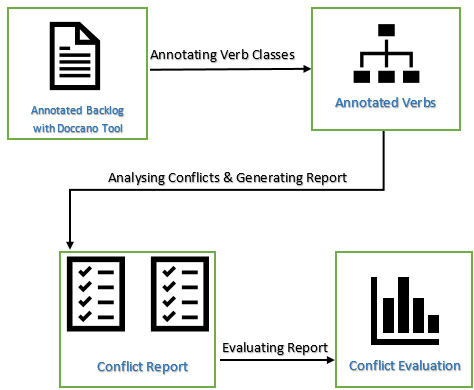
\includegraphics[scale=0.65]{conflict_operational_flow}
	\caption{Step-by-step visualisation of the tool chain and its inputs and outputs}\label{fig:conflict_operational_flow}
\end{figure}
\paragraph{One-Time-Phase: Creating Database for annotated Verbs}In this phase, each verb should be classified using the VerbNet\footnote{\href{https://verbs.colorado.edu/verbnet}{https://verbs.colorado.edu/verbnet}} classification. Finally, each verb class annotated into four categories, namely \textit{Create, Delete, Preserve, or Forbid} (from now on) called \textit{action-annotation}. 

To validate the action annotations, a personal judgement is made for each verb by three evaluators, so that each person reviews the action annotations for each verb and comments their own action annotation. We then collect all the personal judgements and combine the action annotations for each verb.
%\paragraph{Translating the JSON-Format of the Primary Input}\label{conflict_workflow_preparing_json_format}
%Since the annotated USs in the original JSON files did not split entries such as "Entity", "Action", "Text", "Targets" and "Contains", it is not clear which element belongs to which part of the USs (main or benefit part), which leads to possible ambiguities.

%Accordingly, we use a class called \textit{JSONTransformer} that separates entries based on their occurrence in both the main and benefit parts of the USs. It also specifies an identifier to assign a unique identifier to each US, which is stored in a JSON object called \textit{"US\_Nr"}. 

%These additions improve the system's ability to distinguish and process individual USs within the analytical pipeline.
\paragraph{Conflict Analysis and Extraction of text reports} Creating a text report aims to find conflicts between USs and highlight important information, such as identifying potentially conflict pairs, the conflict reason, the resource (as noun) affected by actions (as verbs) causing the conflict, the texts of the main parts with the affected elements marked with \# and a tabulation of the potentially conflicting pairs.

\paragraph{Evaluating the reports} Once we have created the reports, we can now assess the correctness of the US-pairs reported as conflicts, i.e. whether the reported US-pairs really cause a conflict.

\subsubsection*{Software Architecture}\label{conflict_architectur}
In this section, we present the basic structures of our workflow and the discipline of creating such structures. Each structure comprises software elements, relations among them, and properties of both.
\begin{itemize}
	\item Annotated USs with Doccano Tool\footnote{https://github.com/doccano/doccano}: Mosser et al. used publicly available requirements from Dalpiaz et al.\cite{Dalpiaz2018} consisting of 19 product backlogs and 1,458 USs. The dataset is a raw archive of 19 text files, each containing one US per line. 
	
	As there were no public expert-based annotations, Mosser et al. manually annotated the dataset using the Doccano tool for \textit{Named Entity Recognition}. Labels included persona, action, entity, benefit part and relations such as triggers, targets, and contains based on their domain meta-model.
	
	As artefact we receive a graph-based model with JSON format, which represents the refined and annotated dataset for the recognition of \emph{entities}, \emph{actions}, \emph{personas} and \emph{benefits} of USs \cite{mosser2022modelling}.
	
	\item Eclipse as IDE\footnote{https://eclipseide.org/}: Eclipse is an integrated development environment (IDE) used in computer programming. It contains a base work workspace and an extensible plug-in system for customizing the environment.
	
	\item VerbNet as Verb Lexicon Resource\footnote{https://verbs.colorado.edu/verbnet/}: VN is the largest on-line network of English verbs that links their syntactic and semantic patterns. It is a hierarchical, domain-independent, broad-coverage verb lexicon with mappings to other lexical resource, such as WordNet\footnote{https://wordnet.princeton.edu/}, PropBank \footnote{https://propbank.github.io/}, and FrameNet \footnote{http://framenet.icsi.berkeley.edu/}. 
	
	VerbNet is organized into verb classes extending Levin (1993) classes through refinement and addition of subclasses to achieve syntactic and semantic coherence among members of a class. Each verb class in VN is completely described by thematic roles, selectional preferences of the arguments, and frames consisting of a syntactic description and a semantic representation with subevent structure patterned on the Dynamic Event Model of Pustejovsky and Moszkowicz and Pustejovsky\cite{kipper2006extending}.
	
	\item JSONTransformer Class: This class is part of the \textit{org.henshin. backlogconflict.code.preparation} package and is a key component of the software architecture designed for transforming primary input datasets in JSON format. It separates entries based on their occurrence in both the main and benefit parts of the USs. It also assigns a unique identifier to each US to facilitate tracking and management. 
	
	This transformation simplifies subsequent tasks for editing, analysing and conflict resolution by providing a clear structure for the USs and their components. The separation of main and benefit parts and the assignment of unique identifiers improves the manageability and traceability of USs within the system.
	
	\item Action Annotation Reference Database: This database is essential for identifying conflicts between USs, especially conflicts arising from actions over common entities ( as resources). To achieve this, we categorise verbs into four different groups namely \textit{Preserve, Delete, Create, and Prohibit}.
	
	The main purpose of the action Annotation reference database is to facilitate the translation of actions (in the form of verbs) found in USs into corresponding action-annotations. This process involves several important steps:
	\begin{enumerate}
		\item Collection of Actions: We collect all actions (represented as verbs) from existing datasets and compile them into a CSV file. This file serves as comprehensive reference database.
		
		\item Contextual Translation: Each verb in the CSV file is translated into the corresponding action-annotations related to its VerbNet class. 
		
		\item Personal Judgement: To validate the action annotations, three evaluators individually assess each verb. Each evaluator reviews the annotations and provides their own comments. We then gather these individual assessments and combine them to finalize the action annotation reference database for each verb.
	\end{enumerate}
	
	\item VerbFinder Class: The \texttt{VerbFinder} class is an essential component within the \textit{org.henshin.backlogconflict.code.preparation} package, designed to interface with the action annotation database and facilitate the process of mapping verbs to their corresponding action annotations. 
	
	\item ActionsAnnotationsCreator class : This class is a component within the \textit{org.henshin. backlogconflict.code.preparation} package. Its primary function is to improve the JSON transformation process by incorporating action annotations into the JSON dataset. 
	
	The class adds entries that consist of a set of triples: "action", "entity", and "action-annotations". These action-annotations are sourced from the reference database, which ensures that conflict detection and resolution are consistent and accurate. The matching process is done using the \texttt{VerbFinder} class. 
	
	\item ReportMaker Class: This class developed within the \textit{org.henshin.backlogconflict .code.report} packages, its primary function is to identify conflicting US-pairs based on specific criteria and generate comprehensive reports on these conflicts. It performs the following key tasks:%This class provides detailed information on the nature of the conflicts, making it an invaluable tool for maintaining system coherence and resolving inconsistencies. 
	\begin{enumerate}
		\item Identification of Conflict US-pairs: The class analysis USs to identify pairs that conflict based on predefined criteria. These criteria including conflicting actions, or inconsistencies in the USs.
		
		\item Detailed Conflict Reporting: Once conflicts are identified, the class generates detailed reports. These reports contain essential information such as the affected entity(as resource), potential conflicted actions, conflict reason, and the texts of main parts of the USs with marked elements with hash symbol (\#).
		
		\item Tabular Summary: In addition to detailed conflict descriptions, the class also produces a tabular summary of all identified conflict pairs in a backlog, providing a quick overview of the conflict US-pairs.
	\end{enumerate}

	
\end{itemize}
Figure \ref{fig:conflict_technical_implementation} shows the architectural composition, highlighting the integral components and their user interface and artefacts.
\begin{figure}[h]
	\centering 
	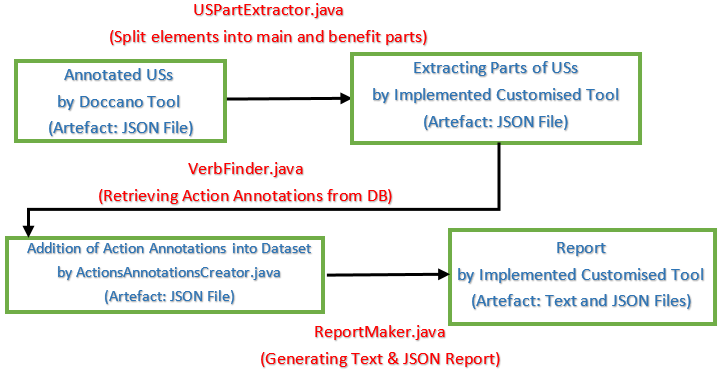
\includegraphics[scale=0.6]{conflict_technical_implementation}
	\caption{Design phases}\label{fig:conflict_technical_implementation}
\end{figure}
Regarding conflict, some definitions are clarified:
\begin{definition}[\textbf{Customized User Story}]
	In order to apply conflict analysis to the backlog, a customized user story is defined, which consists solely of the main part that collectively describes what the user wants and the consequences of this need for the resources.
\begin{itemize}
	\item The \textit{main part} is essential as it clearly and concisely summarizes the persona, the intended functionality, and the resources required to perform the action. This part usually follows the format: \textit{"As a [persona], I want [actions over entities]."}
	
	In this customized US, the intended functionality, which describe the action that the persona wants to perform or the function they need, will be transformed into four annotations: "create," "delete", "preserve", or "forbid". These annotations serve to standardize the actions for conflict analysis:
	
	\begin{itemize}
		\item \textbf{Create:} This action-annotation describes the introduction or addition of a new entity within the system. For example, the action "apply" in US \textit{"As a staff member, I want to apply for a hold."} is annotated with "create" action.
		
		\item \textbf{Delete:} This action-annotation indicates the removal or elimination of an entity from the system. For example, the action "remove" in US \textit{"As a staff member, I want to remove a hold."} is annotated with "delete" action.
		
		\item \textbf{Preserve:} This action-annotation involves safeguarding, or using an existing entity without alterations. For example, the action "browse" in US \textit{"As a researcher, I want to browse through files in a collection."} is annotated with "preserve" action.
		
		\item \textbf{Forbid:} This action-annotation specifies prohibiting certain actions on an entity. For example, the action "restrict access" in US \textit{"As a collection curator, I want to restrict access to my collection or items to duke IP addresses."} is annotated with "forbid" action.
	\end{itemize}
	
	Specifying the resources required to perform the action helps with planning and resource allocation, ensuring that the development team is aware of the tools, technologies, and time required. This includes identifying all entities involved in the actions described and their relationships.
	
	In other words, with respect to the action, we translate it into the aforementioned action-annotations for conflict analysis. This translation standardizes the actions, making it easier to identify and resolve conflicts between USs.
	
	It is worth noting that in this form of US, the benefit part is not considered as part of the structure of USs. The focus is solely on the actions and resources, simplifying the US to its core components necessary for conflict analysis.

\end{itemize}
\end{definition}
\begin{definition}[\textbf{Conflict}]
	Conflict refers to situations where two USs try to:	 
	\begin{itemize}
		\item delete a resource which another US are using
		\item delete a resource which another US also wants to delete
		\item create a resource which another US prohibits
	\end{itemize}
	$Notation$. Lowercase identifiers refer to single elements, and uppercase identifiers denote sets. 
	\\A user story is a 1-tuple $us = \langle m\rangle $ where:
	\begin{itemize}
		\item A main $m$ is define a 6-tuple: \\\\$m = \langle p,A,E,Tr,Ta,Co\rangle $ \\\\where:
		
	\begin{itemize}
		\item $p$ is the persona.
		
		\item $A = \{ a_1,a_2,...\} $ is a set of actions.
		
		\item $E = \{e_1,e_2,...\}$ is a set of entities.
		
		\item $Tr = \{(p_1,a_1),(p_2,a_2),...\}$ is a set of trigger references, each begin a pair of persona and action.
		
		\item $Ta = \{(a_1,e_1,R_1),(a_2,e_2,R_2),...\}$ is a set of target references, each begin a triple of action, entity, and action-annotations $R$.
		
		\item $Co = \{ (e_{c1},e_{c2},R_{c1}),(e_{c*},e_{c*},R_{c2}),... \}$ is a set of contain references, each begin a triple of two entities and action-annotations R.
		
		\item $R = \{preserve, create, delete, forbid\}$ are the annotations applied to actions.
	\end{itemize}
	
	\end{itemize}
	To denote that a syntactic operator, we add the subscript
	“syn”; for instance, $=_{syn}$ is syntactic equivalence which introduced by Lucassen et al. \cite{lucassen2016improving}.\\ Consider two USs:\\\\ $us_1 = \langle m_1\rangle $ where $m_1 = \langle p_1,a_1,e_1,tr_1,ta_1,co_1 \rangle$ \\\\$us_2 = \langle m_2\rangle$ where $m_2 = \langle p_2,a_2,e_2,tr_2,ta_2,co_2 \rangle$ and $co_2 = (e_{c1},e_{c2},R_{c1})$\\\\
	$us_1$ causes a conflict if:
	\begin{enumerate}
		\item The entity $e_1$ is an exact redundant of entity $e_2$, formally:\\ $isRedundant(e_1,e_2) \leftrightarrow e_1 =_{syn} e_2$ and one of the following conditions holds:\\
		\begin{enumerate}
			\item $ta_1 = (e_1,a_1,"preserve")$ and $ta_2 = (e_2,a_2,"delete")$
			
			\item $ta_1 = (e_1,a_1,"create")$ and $ta_2 = (e_2,a_2,"forbid")$
			
			\item $ta_1 = (e_1,a_1,"delete")$ and $ta_2 = (e_2,a_2,"delete")$
		\end{enumerate}
		
		\item The entity $e_1$ is an exact redundant of  $e_{c1}$, formally:\\ $isRedundant(e_1,e_{c1}) \leftrightarrow e_1 =_{syn} e_{c1}$ and one of the following conditions holds:\\
		\begin{enumerate}
			\item $ta_1 = (e_1,a_1,"preserve")$ and $co_2 = (e_{c1},e_{c2},"delete")$
			
			\item $ta_1 = (e_1,a_1,"create")$ and $co_2 = (e_{c1},e_{c2},"forbid")$
			
			\item $ta_1 = (e_1,a_1,"delete")$ and $co_2 = (e_{c1},e_{c2},"delete")$
		\end{enumerate}
	\end{enumerate}
	 
	To comprehensively assess conflicts, it is important to consider not only the textual content but also the functional relevance of each action over entities within the USs. By categorizing actions into four groups, conflict that may not be immediately apparent through a simple text comparison can be uncovered, thereby reducing time consumed in finding conflicts manually.
\end{definition}	


\subsubsection*{Design Phases}\label{design_phases}
To provide a comprehensive overview of the design phases, this section explains each step of the process, from initial setup to final evaluation, using practical examples.
\subsubsection*{Step 1: Data Preparation}\label{design_step_1}
As primary input, we receive a graph-based model generated by the Doccano tool, which represents the refined and annotated dataset for the recognition of \emph{entities}, \emph{actions}, \emph{persons} and \emph{benefits} of USs \cite{arulmohan2023extracting}.

The datasets have the JSON format, the structure of which is very important in the Java classes \textit{RuleCreator}, \textit{ReportExtractor}, and \textit{Evaluation}. Therefore, understanding the JSON format provided is needed for the further procedure.

Each JSON file for a backlog dataset contains a JSON-array in which each US entry is defined as a JSON-object. Listing \ref{list:desing_json_format} illustrates the format used for the US entry.
\begin{MyListing}
	\paragraph{}
	\hrule
	\centering
	\lstinputlisting[basicstyle=\ttfamily\footnotesize]{Listing/json_format.json}
	\caption{The JSON format of each US entry in JSON file}\label{list:desing_json_format}
	\hrule
\end{MyListing}
Mosser et al. have linked each \emph{Persona} to each \emph{Primary Action} as \emph{Trigger} relationships, each \emph{Primary Actions} to each \emph{Primary Entity} as \emph{Target} relationships and each \emph{Primary/Secondary Entity} to each \emph{Primary/Secondary Entity} implying a \emph{Contains} relationship\cite{arulmohan2023extracting}.

To interact with the entries in JSON file, we need to distinguish between the entries that are defined as JSON-objects, such as: {Text, Action, Entity, Benefit} and the entries that are defined as a JSON-array, such as: {Persona, Primary/Secondary Action, Primary/Secondary Entity, Triggers, Targets, Contains}.
\subsubsection*{Identifying USs in JSON-File}\label{desing_workflow_nummerize_us}
Annotated USs in each JSON file have no identifier. To distinguish USs, we use a Python script called \textit{nummerise\_us.py} \footnote{https://github.com/amirrabieyannejad/Redundancy\_Analysis/tree/main/Script/numberise\_us}, which receives JSON files as input and adds a JSON object named \enquote{US\_Nr} with an identifier as value (e.g. user\_story\_01) to each US and returns the JSON files as output.
Listing \ref{list:desing_json_format_sample} illustrates the added JSON object "US\_Nr" and its value in the JSON file.
\begin{MyListing}
	\paragraph{}
	\hrule
	\centering
	\lstinputlisting[basicstyle=\ttfamily\footnotesize]{Listing/json_format_sample.json}
	\caption{The JSON format with the additional JSON object "US\_Nr" and its value}\label{list:desing_json_format_sample}
	\hrule
\end{MyListing}
\subsubsection*{Step 2: Creation of Rules}\label{design_step_2}
Step 2 of the design involves a central process in which the US data structured in JSON files is transformed into transformation rules using the Henshin API. This involves the creation of an Ecore meta-model that represents the structure of the data we are working with, followed by the generation of Henshin transformation rules using RuleCreator class.
\subsubsection*{Creating Ecore Meta-Model}\label{design_workflow_ecore}
To be able to create rules in Henshin, an Ecore (meta)-model should be available. Ecore is the core (meta)-model at the heart of the EMF (Eclipse Modelling Framework). It enables the formulation of other models by utilising its constructs.

Accordingly, we create an Ecore meta-model as shown in Figure \ref{fig:design_ecore_meta_model}, which is inspired by the meta-model shown in Figure \ref{fig:conceptual_metamodel} and corresponds to the JSON-objects in the JSON-file as follows:
\begin{itemize}
	\item \textit{Persona} as a class in the meta-model corresponds to the JSON-object \enquote{Persona} in the JSON-file.
	\item \textit{Entity} as an abstract class, from which \textit{Primary/Secondary Entity} inherits as a class in the meta-model, corresponds to the JSON-object \enquote{Entity}, which contains two JSON-arrays, namely \enquote{Secondary/Primary Entity} in the JSON-file.
	\item \textit{Action} as an abstract class and \textit{Primary/Secondary Action} as an inherited class in the meta-model correspond to the JSON-object \enquote{Action}, which contains two JSON-arrays, namely \enquote{Secondary/Primary Action} in the JSON-file.
	\item \textit{Benefit} as a class in the meta-model, which also has an attribute called \enquote{text} that corresponds to the JSON-object \enquote{Benefit} in the JSON-file.
	\item \textit{Story} as a class in the meta-model that contains text from US, which also has an attribute called \enquote{text} that corresponds to the JSON-object \enquote{Text} in the JSON-file.
	\item Abstract class \textit{NamedElement} has attribute \textit{name}, which Primary/Secondary Action/Entity inherit from it, which corresponds to the value of \textit{Primary/Secondary Action/Entity} in JSON-file.
	\item \textit{Edge} with the name \textit{triggers} between Persona and Primary Action in the meta-model, which corresponds to the JSON-array \enquote{Triggers}, where each JSON-array in it contains a pair, the first element corresponding to the \textit{Persona} and the second to the \textit{Primary Action}.
	\item \textit{Edge} named \textit{targets} between Primary/Secondary Action and Primary/Secondary Entity in the meta-model, which corresponds to the JSON-array \enquote{Targets}, where each JSON-array has a pair, the first element corresponding to \enquote{Primary/Secondary Action} and the second element corresponding to \enquote{Primary/Secondary Entity}.
	\item \textit{Edge} named \textit{contains} between Primary/Secondary Entity and itself in the meta-model, which corresponds to the JSON-array \enquote{Contains}, where each JSON-array in it has a pair where the first element corresponds to \enquote{Primary/Secondary Entity} and the second element corresponds to \enquote{Primary/Secondary Entity}.
\end{itemize}
\begin{figure}[h]
	\centering
	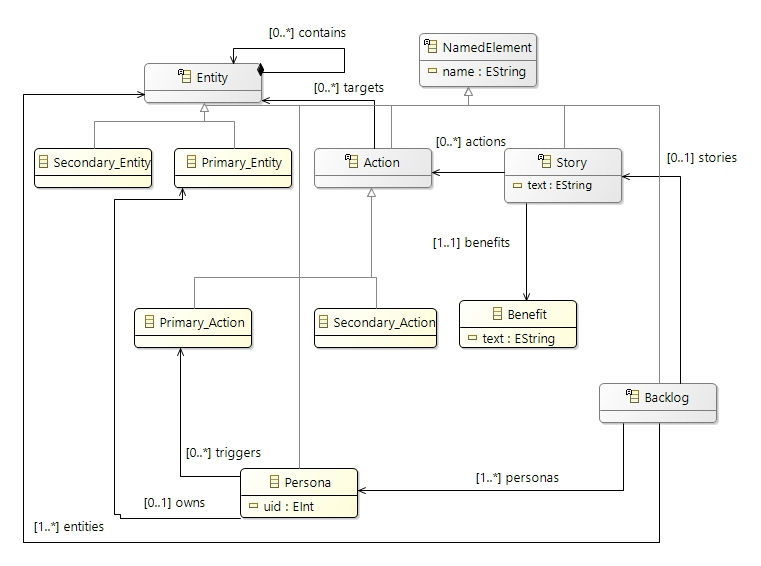
\includegraphics[scale=0.6]{ecore_metamodel}
	\caption{Ecore meta-model inspired by Mosser et al. \cite{mosser2022modelling}}\label{fig:design_ecore_meta_model}
\end{figure}
\subsubsection*{Creating Rules}\label{design_workflow_rule_creator}
With the identified USs in the the JSON-file, we generate rules with the Henshin package \textit{org.eclipse.emf.henshin.model.compact}, which is responsible for the creation of \textit{transformation rules} and their \textit{classes}, \textit{attributes}, \textit{edges} and annotates them with \textless\emph{Delete}\textgreater, \textless\textit{Create}\textgreater or\textless\textit{Preserve}\textgreater, which are vital for the CDA tool to recognise the redundant pairs.

To generating rules we create a package named \textit{org.henshin.backlog.code.rule} and specially the class \textit{RuleCreator} which used following classes\footnote{https://wiki.eclipse.org/Henshin/Compact\_API}:
\begin{itemize}
	\item \textit{org.eclipse.emf.henshin.model.compact.CModule}: CModule class can import elements from an Ecore file to use them in the transformation process responsible for linking the Ecore meta-model to the Henshin-file to be created.
	\item \textit{org.eclipse.emf.henshin.model.compact.CRule}: Once we have a CModule, we can specify transformation rules with the CRule class and create them.
	\item \textit{org.eclipse.emf.henshin.model.compact.CNode}: Now that we have a transformation rule, we want to fill this rule with nodes, edges and attributes. To create a node within a transformation rule, we need the CRule class. To create an edge we need to reference two nodes together. The default action when specifying a node, edge or an attributes is the \textless\emph{preserve}\textgreater action. We can also specify a different action when we create a node or an edge, for example \textless\emph{delete}\textgreater or\textless\emph{create}\textgreater.
	\item org.henshin.backlog.code.rule.RuleCreator: We implement \textit{RuleCreator} class that creates a rule with annotated nodes, edges and attributes based on a JSON-file as input and a Henshin-file containing all rules as output, where each rule and its members(nodes, attributes, edges) correspond to the individual US and their JSON-objects/arrays in the JSON-file. 
	
	The most important design decision of this class is the way nodes, attributes and edges are annotated in order to be able to apply conflict and dependency analysis (CDA) for rules stored as a Henshin file.
	
	We decided to annotate the \enquote{name} attribute of all Primary/Secondary Actions/Entities and their associated edges including \enquote{targets}, \enquote{triggers} and \enquote{contains} as \textless delete\textgreater  action. 
	
	The main goal is to increase the probability of identifying US-pairs characterised by matching names of \textit{action} nodes and \textit{entity} nodes in conjunction with an edge called \textit{targets}. This congruence serves as a basic criterion for identifying potentially redundant US-pairs and simplifies the process of redundancy detection in the context of US analysis.
\end{itemize}
\begin{example}
	Listing \ref{list:design_json_user_story_12} shows the JSON format in relation to user\_story\_12 and Figure \ref{fig:desing_rule_user_story_12} shows the application of the RuleCreator class in this US, which is a transformation rule where the targets and the associated contains relationships are annotated as a \textless Delete\textgreater action and the rest of the nodes and edges are annotated as a \textless Preserve\textgreater action.\\\\
	Text of US is:
	user\_story\_12: "\#G03\# As a Staff member, I want to Assign an Application for Detailed Review, so that I can review the for compliance and subsequently approved or denied."
	%Considering the backlog dataset as shown in Listing \ref{list:backlog_g03}:
	\begin{MyListing}
		\paragraph{}
		\centering
		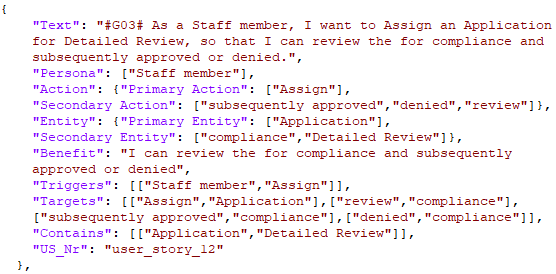
\includegraphics[scale=0.8]{Listing/json_user_story_12.png}
		\caption{JSON entities Related to user\_story\_12}\label{list:design_json_user_story_12}
	\end{MyListing}
	\begin{figure}[h]
		\centering
		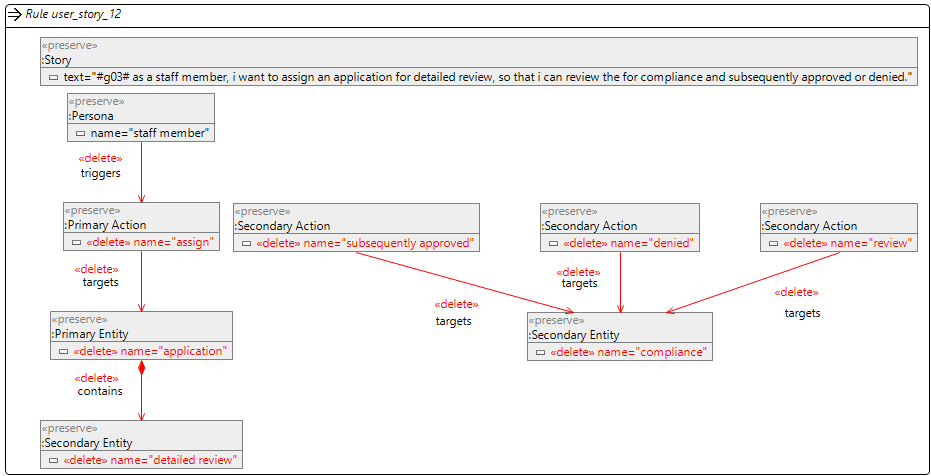
\includegraphics[scale=0.6]{rule_user_story_12}
		\caption{Generated transformation rule related to user\_story\_12 using RuleCreator class}\label{fig:desing_rule_user_story_12}
	\end{figure}
	As we can see, the "targets" edges and their direct relationships ("triggers" and "contain", if any) are also annotated as \textless delete\textgreater, which is very important to find redundant elements with the CDA tool.
\end{example}
\begin{example}
	Listing \ref{list:design_json_user_story_39} shows the JSON entities related to user\_story\_39 and Figure \ref{fig:design_rule_user_story_39} shows transformation rule generated by RuleCreator class.\\\\
	Text of US is:
	user\_story\_39: "\#G03\# As a Plan Review Staff member, I want to Review Plans, so that I can review them for compliance and either approve, or fail or deny the plans and record any conditions, clearances, or corrections needed from the Applicant."
	\begin{MyListing}
		\paragraph{}
		\centering
		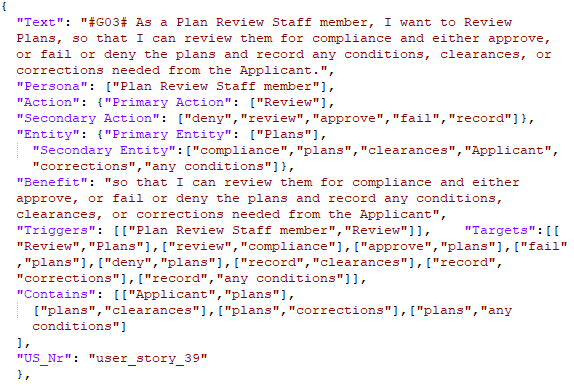
\includegraphics[scale=0.8]{Listing/json_user_story_39.png}
		\caption{JSON entities Related to user\_story\_39}\label{list:design_json_user_story_39}
	\end{MyListing}
	\begin{figure}[h]
		\centering
		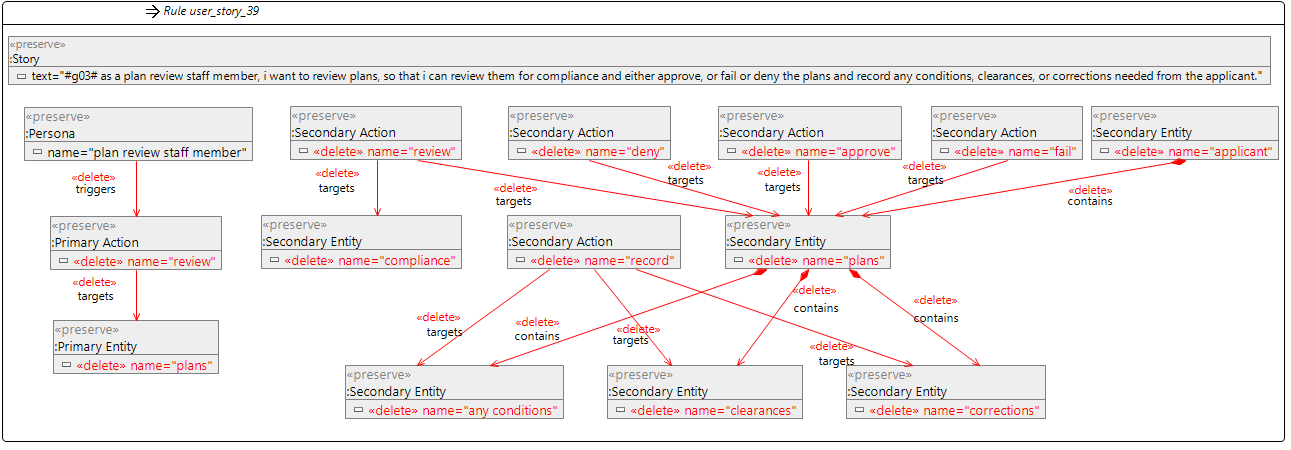
\includegraphics[scale=0.43]{rule_user_story_39}
		\caption{Generated transformation rule related to user\_story\_39 using RuleCreator class}\label{fig:design_rule_user_story_39}
	\end{figure}
	Attribute "Plan", as we can see, it appears both in the main part as a primary entity and in the benefit part as a secondary entity, forming the various relationships as targets and contains.
\end{example}
\begin{example}
	Listing \ref{list:desing_json_user_story_51} shows the JSON entities related to user\_story\_51 and Figure \ref{fig:desing_rule_user_story_51} shows transformation rule generated by RuleCreator class.\\\\
	Text of US is:
	user\_story\_51: "\#G03\# As an Enforcement Staff member, I want to Issue a Notice of Violation, so that I can provide formal communication to the responsible party."
	\begin{MyListing}
		\paragraph{}
		\centering
		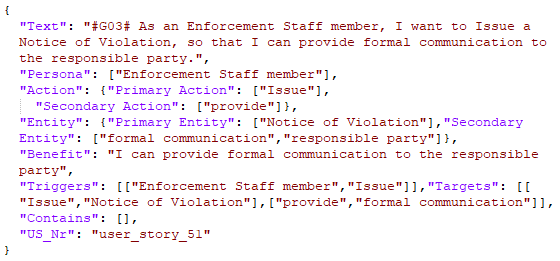
\includegraphics[scale=0.8]{Listing/json_user_story_51.png}
		\caption{JSON entities Related to user\_story\_51}\label{list:desing_json_user_story_51}
	\end{MyListing}
	\begin{figure}[h]
		\centering
		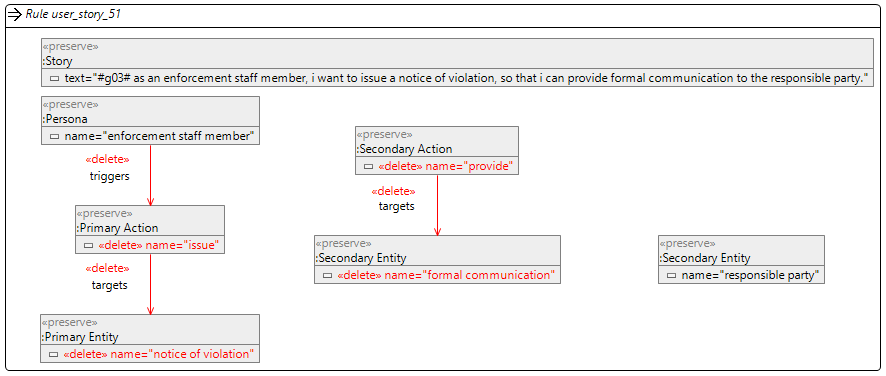
\includegraphics[scale=0.55]{rule_user_story_51}
		\caption{Generated transformation rule related to user\_story\_51 using RuleCreator class}\label{fig:desing_rule_user_story_51}
	\end{figure}
	Last but not least, we have determined that the secondary entity "responsible party" has neither a target nor a contains relationship. Therefore, it is not annotated as \textless delete\textgreater, but as \textless preserve\textgreater. This is due to the fact that some phrases have been identified as entities in the Doccano tool, but their relationship is not annotated at all, which is problematic for analysing redundancy.
\end{example}
\subsubsection*{Step 3: Conflict and Dependency Analysis}\label{step_3}
After the rules and the corresponding henshin file have been created by the RuleCreator class, we are now able to pass them to the conflict and dependency analysis (CDA) to find potential redundancy pairs.

Since the analysis of conflicts and dependencies related to the \textit{attribute} is not yet considered in the CDA API \footnote{https://wiki.eclipse.org/Henshin/conflict\_and\_Dependency\_Analysis}, we decided to use the user interface (UI) of the CDA extension of Henshin, which supports analysis of conflict and dependencies of rules through the interactive use of CDA.

To apply CDA to Henshin files, we just need to right-click on the Henshin file and select \textit{Henshin} -\textgreater\textit{ conflict and Dependency Analysis} from the context menu as shown in Figure \ref{fig:henshin_context_menu}.
\begin{figure}[h]
	\centering
	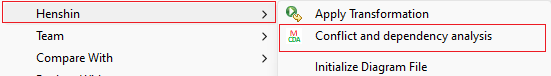
\includegraphics[scale=0.5]{henshin_context_menu}
	\caption{Applying CDA to the selected Henshin file}\label{fig:henshin_context_menu}
\end{figure}
A user interface then appears, prompting to select the rule sets to be analysed and the type of analysis. We then select as \enquote{\textit{First}} and \enquote{\textit{Second} \textit{Rules}}, all rules related to USs. Additionally, as the type of analysis we select \enquote{\textit{conflicts}} as illustrated in Figure \ref{fig:select_rules}.
\begin{figure}[h]
	\centering
	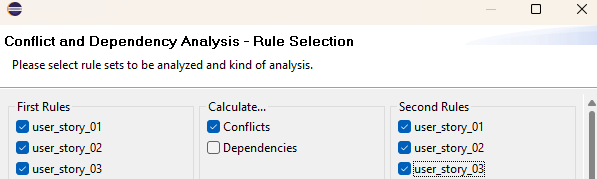
\includegraphics[scale=0.5]{select_rules}
	\caption{CDA user interface: Selection of rules and type of analysis}\label{fig:select_rules}
\end{figure}
On the next page of the CDA UI shown in Figure \ref{fig:select_granularity}, we specify the depth of analysis that we use with \enquote{\textit{Fine granularity}} when selecting \enquote{\textit{Create a complete result table}} and \enquote{\textit{Create an abstract result table}}. 

Fine granularity provides a detailed examination of each conflicting rule by listing all conflict reasons. Unlike coarse granularity, which focuses only on minimal conflict reasons, fine granularity includes both minimal and more general conflict reasons. The binary granularity, where simple conflicting rule pairs are listed, may be too simple for complex systems where understanding the nature of the conflict is essential for the solution. 
We choose \enquote{Fine granularity} as the depth of analysis due to the fact that it shows all conflict reasons for each conflicting rule pair. This allows for a deeper understanding of how different model fragments contribute to conflicts.

A conflict reason is a model fragment whose presence leads to a conflict. General conflict reasons result from different combinations of minimal conflict reasons\cite{cda_api}.
\begin{figure}[h]
	\centering
	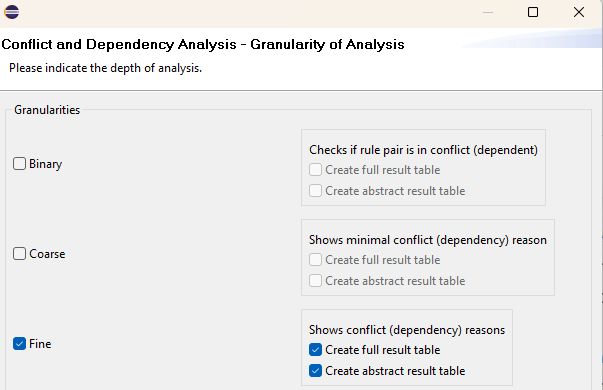
\includegraphics[scale=0.5]{select_granularity}
	\caption{CDA user interface: Selection of report granularity}\label{fig:select_granularity}
\end{figure}
During the execution of the CDA analysis, the rule pairs is analysed and a conflict analysis is performed. Once the calculation is complete, the results are listed in the \enquote{CDA} -\textgreater \enquote{Result window}, as shown in Figure \ref{fig:cda_report}. The top entry shows the granularity, which in our case is \enquote{Fine}. These entries contain the rule pairs that conflict with each other. Each rule pair contains a number of conflict reasons.
\begin{figure}[h]
	\centering
	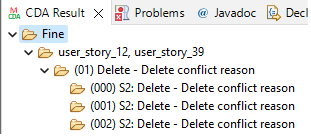
\includegraphics[scale=0.5]{cda_report}
	\caption{CDA report with fine granularity}\label{fig:cda_report}
\end{figure}
Figure \ref{fig:cda_report_in_project_dir} shows how the data is saved in the project tree view. The results directory is created in the directory containing the Henshin that was used for the analyses. The new folder name is the date and time at which the analysis was performed. In contrast to the \enquote{\textit{CDA/Results}} view, this folder contains all conflict reasons and atoms together in a rule pair directory.
\begin{figure}[h]
	\centering
	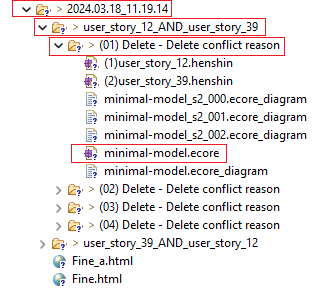
\includegraphics[scale=0.5]{cda_report_in_project_dir}
	\caption{Saving CDA results data in the project structure view}\label{fig:cda_report_in_project_dir}
\end{figure}
For each conflict reason, there is a \enquote{\textit{minimal-model.ecore}} file, that contains packages in which various conflict elements such as \enquote{attributes} and \enquote{references} (edges) are mapped together and displayed in different packages.

Figure \ref{fig:minimal_model_packages} shows the representation of the conflicting attributes and references. An attribute has the property of changing the value and is represented by an arrow \enquote{-\textgreater}. The attribute from the first rule is separated from the second rule by an underscore, just as with the nodes.
\begin{figure}[h]
	\centering
	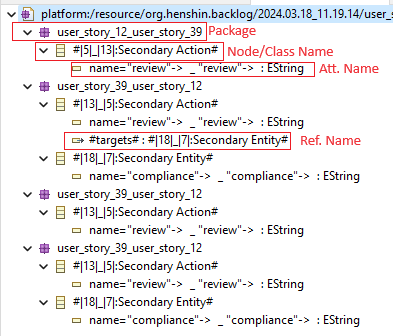
\includegraphics[scale=0.5]{minimal_model_packages}
	\caption{Representation of redundant attributes and references in \textit{minimal-model.ecore} file}\label{fig:minimal_model_packages}
\end{figure}
\begin{example}
	To illustrate this step, we also pass the transformation rules created in step 2, which reflect three USs (user\_story\_12/39/51), to the CDA tool and selecting "conflicts" as conflict type to calculate with "fine granularity" as the depth of analysis.\\
	Once the calculation is complete, the results are listed in the "CDA" -\textgreater "Results Window" as shown in Figure \ref{fig:step_3_cda_report}. Figure \ref{fig:step3_cda_report_project_tree_view} shows how the data is saved in the project's tree view, which contains all conflict reasons and atoms together in a rule pair directory.
	\begin{figure}[h]
		\centering
		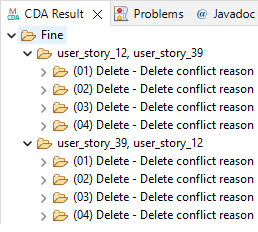
\includegraphics[scale=0.5]{step_3_cda_report}
		\caption{CDA report in relation to three transformation rules with "conflicts" as the type to be calculated and "fine granularity" as the depth of the analysis}\label{fig:step_3_cda_report}
	\end{figure}
	\begin{figure}[h]
		\centering
		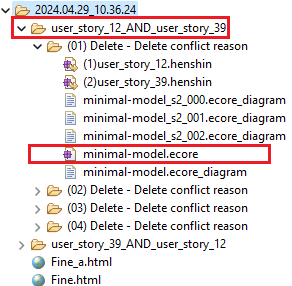
\includegraphics[scale=0.5]{step3_cda_report_project_tree_view}
		\caption{Saving CDA results data in the project's tree view}\label{fig:step3_cda_report_project_tree_view}
	\end{figure}
	As we can see, the CDA tool has only found redundancy between user\_story\_12 and user\_story\_39. This is because there are no redundant clauses between two USs (user\_story\_12 and user\_story\_39) and user\_story\_51.\\
	Regarding the redundant elements specifically, we can refer to the created file "minimal-model.ecore", which is located in the tree view of the project under each conflict reason. Figure \ref{fig:step3_cda_report_project_tree_view} show the minimal-model.ecore file related to user\_story\_12 and user\_story\_39.\\\\
	The file Minimal-model.ecore, which refers to user\_story\_12 and user\_story\_39, is divided into packages, with each package containing different matches of redundant elements. If there is a redundancy between two elements, this is explicitly indicated by a hash symbol (\#). Figure \ref{fig:step3_cda_package} illustrates the redundant elements found in each package.\\\\
	\begin{figure}[h]
		\centering
		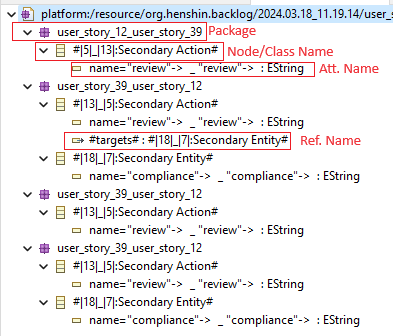
\includegraphics[scale=0.5]{minimal_model_packages}
		\caption{Representation of the redundant elements in each package within \textit{minimal-model.ecore} file}\label{fig:step3_cda_package}
	\end{figure}
	For example, the attribute "name" with the value "review" in "Secondary Action" and the attribute "targets" with the value "compliance" in "Secondary Entity" are labelled as redundant (both with a hash symbol). The reference to "targets" is also marked as redundant (with a hash symbol), which means that the reference (targets) from "Secondary Action" to "Secondary Entity" is also redundant between USs, which is a very important criterion for finding redundancy correctly.
\end{example}
\subsubsection*{Step 4: Report Extraction}\label{step_4}
To create a lightweight report for the group or individual in question, we need to extract the key information from the CDA report, e.g. redundancy US-pair, redundancy clauses, count of redundancy clauses in each part of the US (main or benefit part), and create a report as a text file with the following information:
\begin{itemize}
	
	\item A table of potential redundant pairs with the number of total redundancy clauses.
	
	\item Founded potential redundant US-pairs.
	
	\item Redundancy words and clauses of founded US-pairs. Clauses consisting of two words that have one of the relationships triggers, targets or contains.
	
	\item Text of US-pairs whose redundancy words are marked with a hash symbol (\#).
	
	\item Parts of the sentence in which words and clauses are found.
\end{itemize}
\subsubsection*{Structure of a US}
The delineation and checking of redundancy clauses within USs requires a methodical approach, especially when distinguishing between the main and the benefit part of a US-pair. This distinction is crucial to ensure that redundancy identifications within one part are not mistakenly transferred to the other. Consequently, the analytical framework comprises three conditions, each of which specifies its own methodology for case processing:
\begin{itemize}
	\item Presence of benefit in both USs of the redundancy-pair: if a benefit is identifiable in each US of the pair, a process of separation is used to split the main content from the benefit parts. After this separation, a targeted search for redundancy clauses is carried out only within the main part, whereby identified redundancies are annotated with a hash symbol (\#). This process is repeated for the benefit parts to ensure a thorough check and marking of redundancies within each individual part.
	
	\item Exclusive presence of a benefit in one US of the redundancy-pair: In scenarios where only one US of the pair contains a benefit part, the analysis is limited to the main part of both USs. The aim remains the identification and annotation of redundancy clauses within this part. The lone benefit part remains in its original state and is excluded from the redundancy check.
	
	\item Absence of benefit parts in both USs of the pair: If neither of the two USs of the redundancy-pair contains a benefit part, the focus shifts completely to the main parts. The investigation is designed to highlight redundancy clauses within these parts, whereby the benefit parts are not taken into account due to their non-existence.
	
\end{itemize}
This structured and segmented approach ensures precise and efficient identification of redundancy clauses within the USs, optimising the clarity and effectiveness of textual report.
\begin{example}
	After the CDA directory for user\_story\_12 and user\_story\_39 is created by CDA tool graphic interface (UI), we pass the location of directory into ReportExtractor class and in order to extracting the important information and save it into the texual report as well as JSON report.
	Listing \ref{list:textual_report_sample} illustrates the example of the textual report. In this case, the report only contains one US-pair.
	\begin{MyListing}
		\paragraph{}
		\centering
		%\lstinputlisting[basicstyle=\ttfamily\footnotesize]{Listing/TextualReportSample.txt}
		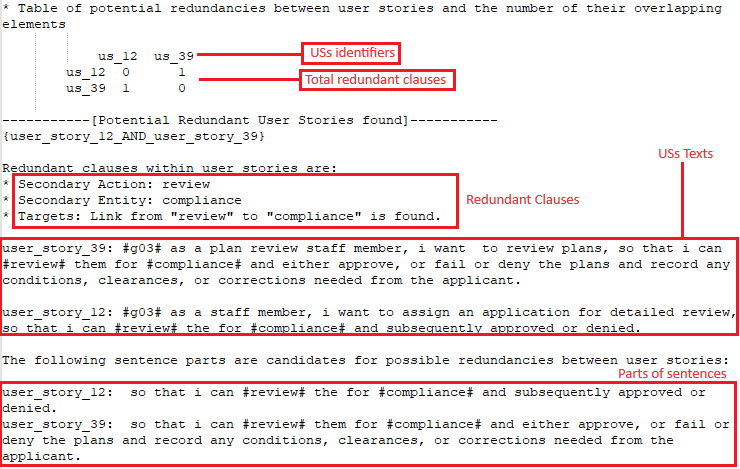
\includegraphics[scale=0.7]{Listing/TextualReportSample.png}
		\caption{Example of generated textual report for one US-pair}\label{list:textual_report_sample}
	\end{MyListing}	
	As we can see, the text report consists of a 2 x 2 table whose first column and first row are US identifiers, and the numbers inside the table are the total number (benefit part + main part) of redundancy elements between two USs; secondly, the redundant clauses related to the redundant US-pair are listed; thirdly, the text of US whose redundant phrases are marked with a hash symbol; finally, the part of the clauses in which redundant elements occur is displayed.	
\end{example}
For further evaluation purposes and easy export of the report to another platform such as Excel, a JSON report is created that collects the information about redundant US-pairs separately in a JSON object with the following entries:
\begin{itemize}
	\item Potential Redundant User Stories:  which has stored the US-pair identifier(e.g. "user\_story\_12\_AND\_user\_story\_39"). 
	
	\item Status: consisting of "Main/Beneift Part Redundancy Clauses" and "Total Redundancy Clauses", which store the count of redundancy clauses in the main and benefit part as well as in the total part of the US.
	
	\item Entity: which can consist of a "Secondary/Primary Entity" and stores the founded redundant entities.
	
	\item Common Targets/Contains: which consists of the "Main Part" and "Benefit Part" entries and only stores the targets/contains relationships that are common between the USs in a particular part of the USs. For example, if there are common redundant targets in the main part of the USs, these are included in the "Main Part" entity of the "Common Targets".
	
	\item Text: consisting of two entries, namely "First UserStory" and "Second UserStory", in which the text of the US-pair whose hash symbol has already been applied in redundant phrases is stored.
	
	\item Project Number: stores the number of the Project(e.g. "G03").
	
	\item Part of Sentence: consists of the entries "First UserStory" and "Second UserStory", in which the part of the US sentences containing redundant clauses is stored.
	
	\item All Targets/Contains: which consists of the "Main Part" and "Benefit Part" entries and stores the whole targets/contains relationships that are occurred in the particular part of the USs.
	
\end{itemize}
\begin{example}
	Listing \ref{list:json_report_sample} illustrates the example of the JSON report regarding user\_story\_12 and user\_story\_39.
\end{example}
\begin{MyListing}
	%\paragraph{}
	
	\centering
	%\lstinputlisting[basicstyle=\ttfamily\footnotesize]{Listing/TextualReportSample.txt}
	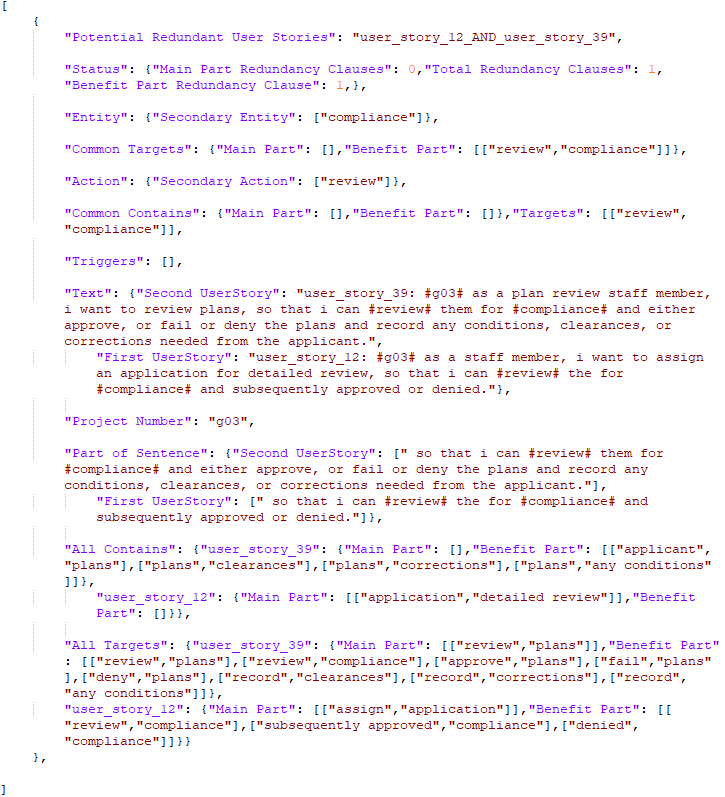
\includegraphics[scale=0.7]{Listing/JSONReportSample.png}
	\caption{Example of generated JSON report for one US-pair}\label{list:json_report_sample}
	
\end{MyListing}	
\subsubsection*{Step 5: Report Evaluation}
The Evaluation class, part of the \textit{org.henshin.backlog.code.evaluation} package, was developed to determine the level of redundancy in USs based on JSON reports. This class provides methods to evaluate whether two USs are either fully or partially redundant, analysing different application components of these USs.

The evaluation process involves a complex logic to determine whether USs are redundant. This includes:
\begin{itemize}
	\item Checking whether the arrays are empty or contain similar elements.
	\item Comparing the individual elements in the arrays for both USs to determine if they fully match (full redundancy) or if they have some common elements (partial redundancy).
\end{itemize}
\begin{example}
	For the two US-pairs of dataset G03, we apply the evaluation class to determine whether there is redundancy in the main or benefit part, and if so, what type of redundancy is recognised(full or partially).\\\\
	As shown in Listing \ref{list:json_evaluation}, four entries are added to the JSON report, namely "Main Partially Redundant", "Benefit Part Fully Redundant",
	"Main Part Fully Redundant", "Benefit Partially Redundant" as "Status" which their value is whether true or false. 
	\begin{MyListing}
		\paragraph{}
		
		\centering
		%\lstinputlisting[basicstyle=\ttfamily\footnotesize]{Listing/TextualReportSample.txt}
		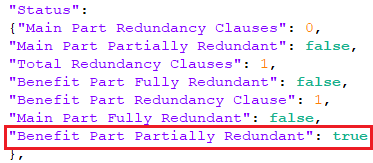
\includegraphics[scale=0.7]{Listing/json_evaluation.png}
		\caption{Example of generated entries in JSON report regarding evaluation of level of redundancy in main or benefit part}\label{list:json_evaluation}
		
	\end{MyListing}	
	
	In the case of user\_story\_12 and user\_story\_39, the entry "Benefit Partially Redundant" was marked as \textit{true}, which means that US-pair in benefit parts are partially redundant.
	
\end{example}
The class performs these checks by iterating through the JSON arrays of Triggers, Targets and Contains and comparing each element with those in the common sections to determine redundancy.


\subsection{Implementation}\label{conflict_implementation}
In this section, we explain the objective and scope of the implementation, the functionality and the programming languages used.

The entire implementation is available in the GitHub repository \footnote{https://github.com/amirrabieyannejad/conflict\_analysis\_between\_USs/tree/main}.
%\subsubsection*{Objective and Scope}
%The goal and scope of the work is divided into four phases. Firstly, converting the USs annotated by the CRF tool into graph transformation rules; secondly, using the CDA tool of the Henshin to automatically report redundancies between USs pairwise; thirdly, extracting important information from the CDA report into a text report; fifthly, evaluation of reports. %For further analysis, we stored the information in a JSON file to be able to import the data into another platform such as Excel.
%Figure \ref{fig:implementation_phases} illustrates the mentioned implementation phases.
%\begin{figure}[h]
%	\centering
%	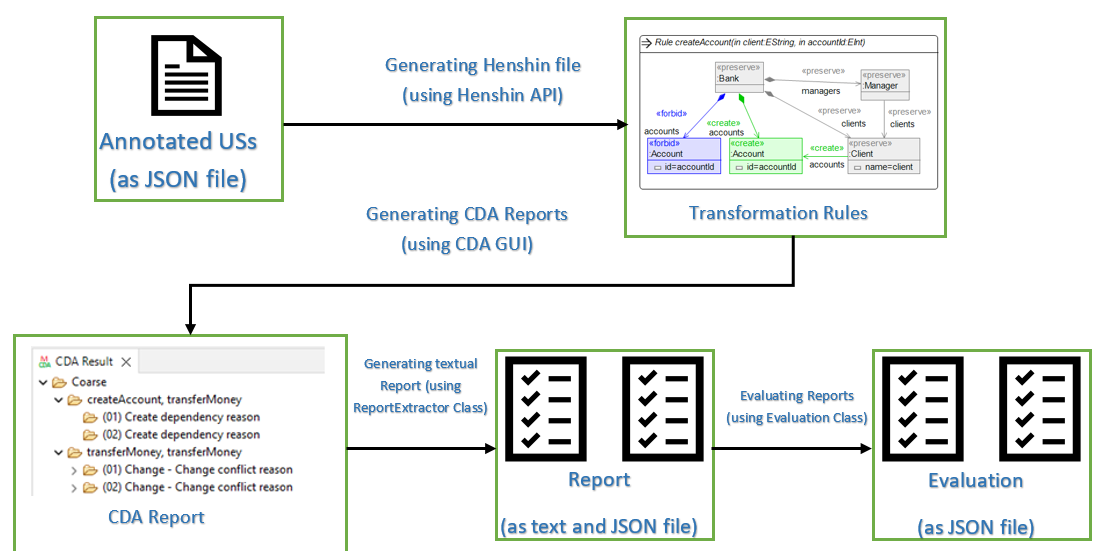
\includegraphics[scale=0.3]{implementation_phases}
%	%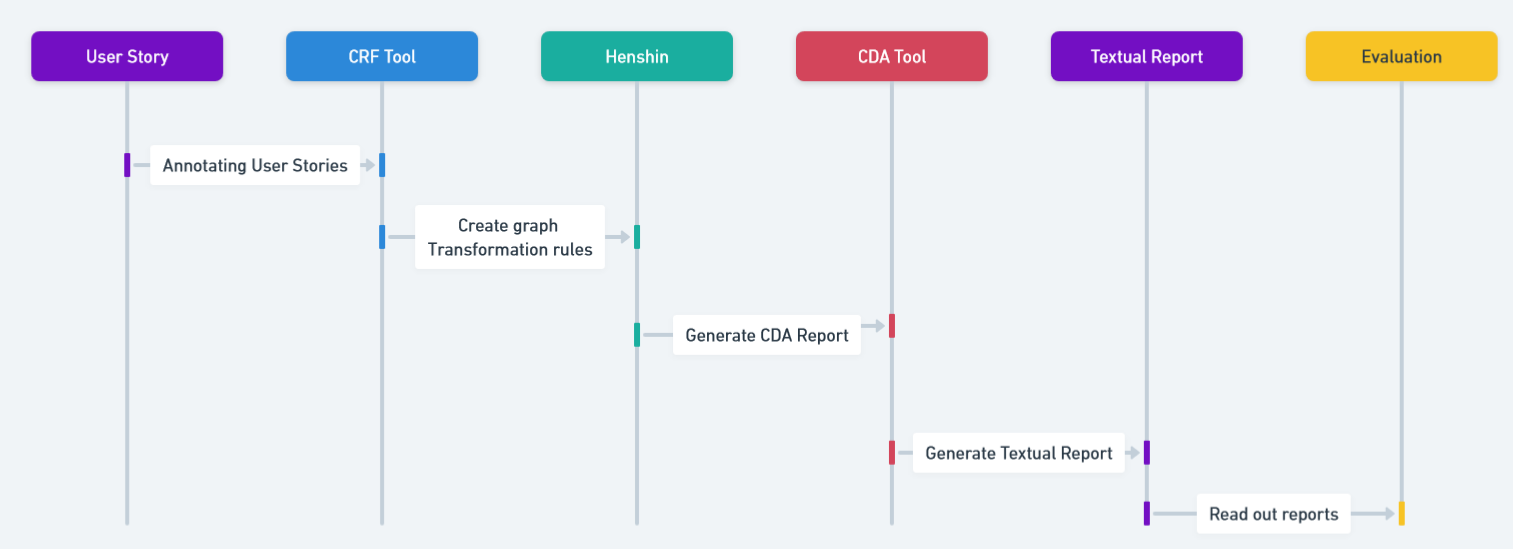
\includegraphics[scale=0.35]{sequence_diagram}
%	\caption{Three Implementation phases}\label{fig:implementation_phases}
%\end{figure} 
\subsubsection*{Methodology}
This section explains and introduces tools that are required during the development process.

Following approach and tools are necessary in order to develop our workflow:
\begin{itemize}	
	\item Java as programming language\footnote{https://www.java.com/de/}: Java is a widely used object-oriented programming language and software platform that is used to implement the Henshin and EMF APIs, which are critical to our approach to utilising them. Therefore, we use Java as our programming language.
	
	\item GitHub as version control\footnote{https://github.com/}: GitHub is a developer platform that allows developers to create, store, manage and share their code. It uses Git software, providing the distributed version control of Git plus access control, bug tracking, software feature requests, task management, continuous integration, and wikis for every project.
\end{itemize} 
\subsubsection*{Implementation Phases}\label{conflict_phases}
This section contains a step-by-step guide to implementation, starting with the set-up and ending with the extracting report.

Following steps implies the classes and methods related to org.backlogconflict.code.preparation:
\subsubsection*{Extracting Parts of USs from the Input Dataset}\label{conflict_step_json_transformer}
In this section, we explain the methods we used to convert the US data structured in JSON files into a custom US data structure that splits the elements such as Entity, Action, Contain, Target in terms of their occurrence in the main and benefit part. 
\subsubsection*{Methods of the USPartExtractor Class}
In this section, the methods of the USPartExtractor class is described as follows:
\begin{itemize}
	
	\item getStringFromOffset: This method was designed to extract a substring from a given main text of US based on the start and end offsets.
	
	As input it receives the text of US, a start offset and an end offset as an integer and as output it extracts the part of the text of US that starts at "start offset" and ends just before "end offset".
	
	\item runUSPartExtractor: This method processes multiple datasets by reading JSON lines from input files, transforming each JSON object, and then writing the transformed JSON objects to output files.
	
	As input it receives:
	\begin{itemize}
		\item An array of dataset names: each name in the array corresponds to a specific dataset that is processed
		
		\item The base directory path in which the dataset files are located. This path is used to construct the full file paths for reading inputs and writing outputs.
	\end{itemize}	
	It iterates through each dataset name in the "dataSets" array and constructs the paths of the input and output file based on the dataset name of the "filePath".
	
	It also reads all lines from the input file and passes them to the \texttt{transformJson} method for the transformation process. Finally, it writes the result to the output file.
	
	\item transformJson: This method is the main component of the USPartExtractor class. It processes a JSON object that represents a US, extracts and categorises its entities and relationships according to their occurrence in the main or benefit part of the US text and assigns this information in a new JSON structure.
	
	As input it receive the original JSON object containing information about a US, including text, entities, and relations.
	
	In this method following steps were carried out:
	\begin{itemize}
		\item It initialize a JSON object to hold the transformation data and extract the basic information like "Text" and "ID" of US as well as "PID"(project ID)
		
		\item It initialises two JSON objects, namely \texttt{Main} and \texttt{Benefit}, and specifies the elements and their relationships accordingly.
		
		\item It initialises JSON arrays for various elements such as "Persona", "Entity", "Action" and splits them based on the start and end offsets of the benefit part into "Main" or "Benefit" JSON object.
		
		If the end offset of an element is smaller than the start offset of the benefit string, it is considered to be an element of the main part, otherwise it is considered to be an element of the benefit part.
		
		\item Iterates through each relation and determines the elements involved. If both elements belong to the main part, a relation is initialised in the "Main" JSON object according to their category (Triggers, Targets, or Contains). 
		
		If both elements belong to the benefit part, a relation is initialised in the "Benefit" JSON object according to their category (Triggers, Targets, or Contains). 
		
		If elements belong to different parts of US, the relation is initialised in a \texttt{Mix} JSON object.
		
	\end{itemize}
	As output a JSON object containing the transformed data will be returned.
\end{itemize}
\subsubsection*{Addition of Action Annotations into Dataset}\label{conflict_action_annotation}
In this section, we explain the classes and their methods that we used to retrieve action annotations associated with the verb from the action annotation database using \textit{VerbFinder} class. Finally, we insert the retrieved action annotations into the JSON structure of the US using \textit{ActionsAnnotationsCreator} class.
\subsubsection*{Methods of the VerbFinder Class}
In this section, the methods of the VerbFinder class is described as follows:
\begin{itemize}	
	\item loadCSV: This method reads a CSV file with verb and action annotation pairs, processes each line and fills a map with these pairs so that when the VerbFinder class is initialised, a map with verb and action annotation pairs is available to retrieve the action annotations as needed.
	
	It receives a file path of the CSV file to be read as input. The method does not return a value directly.
	
	\item getActionAnnotations: This method retrieves the action annotations associated with a specific verb from a pre- populated map (verbMap).
	
	As input, it receives a verb as a string for which the action annotations are to be retrieved.
	
	The method then accesses the verbMap and uses the verb provided as a key.
	
	As output, it receives the corresponding action annotation from the map. If the verb is not available in the verbMap, the method returns \texttt{null}.
	
\end{itemize}
\subsubsection*{Methods of the ActionsAnnotationsCreator Class}
In this section, the methods of the ActionsAnnotationsCreator class is described as follows:
\begin{itemize}	
	\item addActionsAnnotations: This method reads JSON files for each dataset, initialize the VerbFinder with provided file path, adds action annotations to each JSON object correspond to specific US within these files, and saves the modified JSON objects back to the files.
	
	As input it receives:
	\begin{itemize}
		\item An array of dataset names: each name corresponds not only to a subdirectory containing a JSON file to be processed, but also to the file name. 
		
		\item The base directory path in which the dataset files are located. This path is used to construct the full file paths for reading inputs and writing outputs.
		
		\item The base directory path where the CSV file is located. This path is used to build the full file paths for reading the database with the action annotations to initialise the map(verbMap).
	\end{itemize}
	
	The method does not return any value. Instead, it modifies the JSON files in place by adding action annotations to each JSON object related to specific US in the file.
	
	\item addActionAnnotations: This method processes a JSON object that corresponds to a US in order to add action annotations to the "Targets" and "Contains" relationships within the "Main" part of the US in JSON object.
	
	As input, it receive a JSON object representing a US with nested structures for "Main" and "Benefit" part, each containing "Targets", "Contains" arrays.
	
	The method modifies the JSON object by adding the action annotations to the "Targets" and "Contains" relations within the "Main" part.
		
	\item findActionsAnnotations: This method retrieves the action annotation associated with a given verb. This method act as a utility for mapping verbs to their corresponding action annotations using the instance VerbFinder class.
	
	As input, it takes the verb for which the action annotation is to be found. The output returned is a String containing the action annotations for the verb provided.	
\end{itemize}

Figure \ref{fig:conflict_prepration_package_class_diagram} is a class diagram that illustrates the attributes, operations and relationships related to the org.backlogconflict.code.preparation package.
\begin{figure}[h]
	\centering
	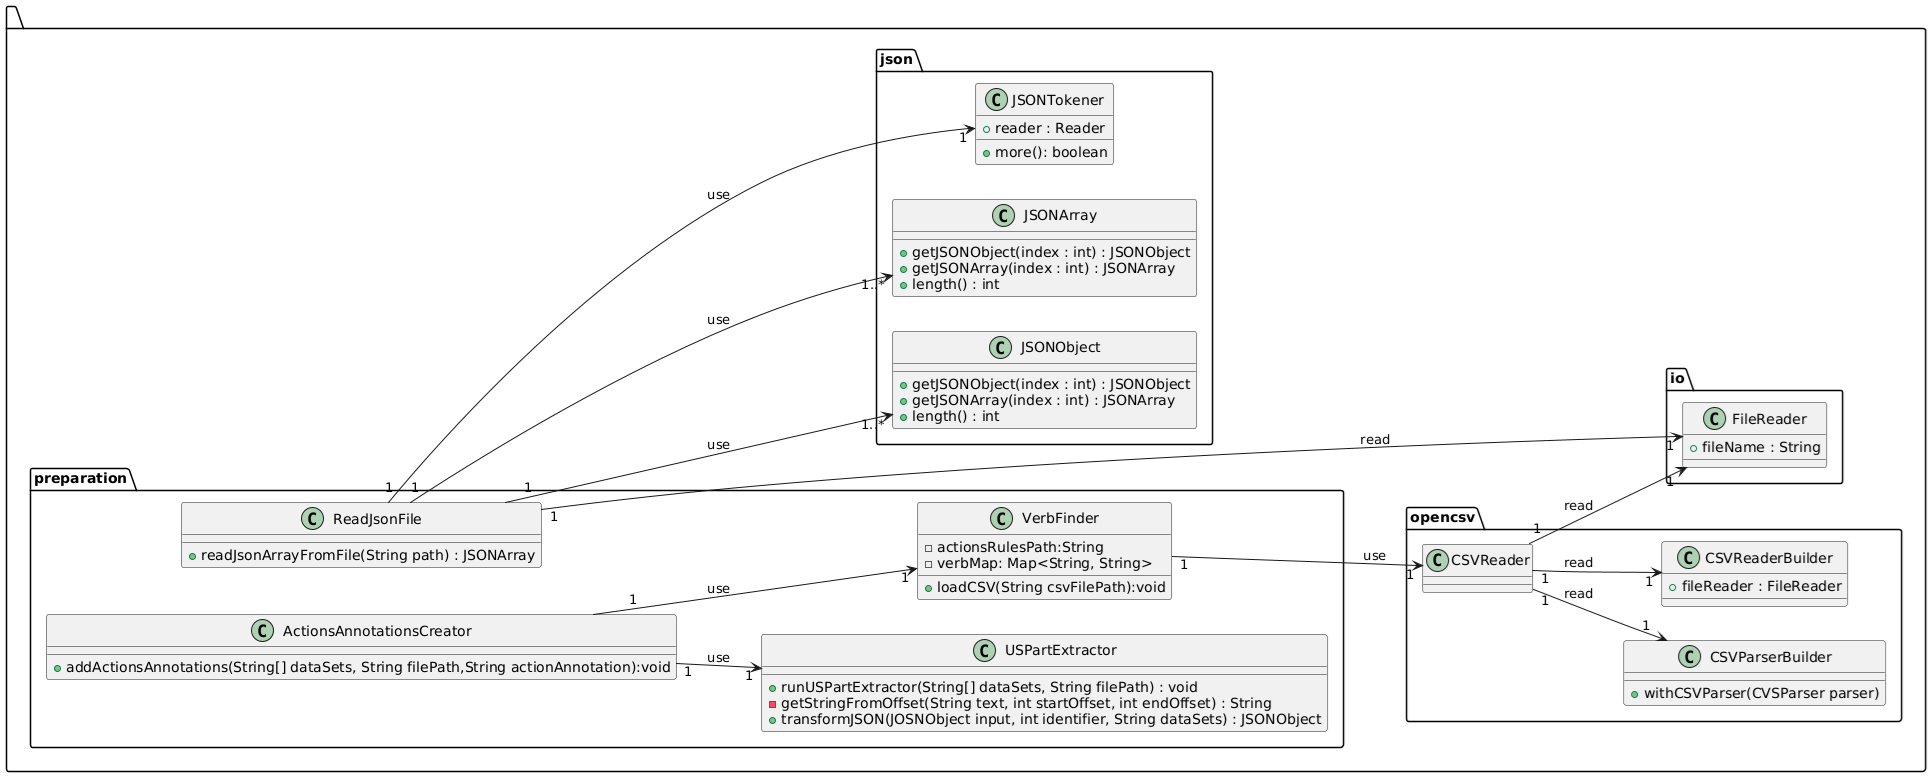
\includegraphics[scale=0.3]{conflict_prepration_package_class_diagram}
	\caption{Class diagram of the org.backlogconflict.code.preparation class and its relationships}\label{fig:conflict_prepration_package_class_diagram}
\end{figure}
%To illustrate this step, three example is given in which the RuleCreator class is applied to a dataset (G03) with three collected USs and the resulting artefact is presented.
%\begin{example}
%Listing \ref{list:json_user_story_12} shows the JSON format in relation to user\_story\_12 and Figure \ref{fig:rule_user_story_12} shows the application of the RuleCreator class in this US, which is a transformation rule where the targets and the associated contains relationships are annotated as a \textless Delete\textgreater action and the rest of the nodes and edges are annotated as a \textless Preserve\textgreater action.\\\\
%Text of US is:
%user\_story\_12: "\#G03\# As a Staff member, I want to Assign an Application for Detailed Review, so that I can review the for compliance and subsequently approved or denied."
%Considering the backlog dataset as shown in Listing \ref{list:backlog_g03}:
%\begin{MyListing}
%	\paragraph{}
%	\centering
%	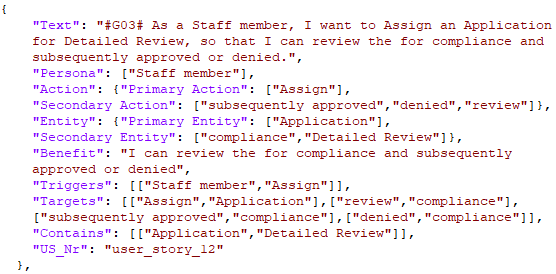
\includegraphics[scale=0.8]{Listing/json_user_story_12.png}
%	\caption{JSON entities Related to %user\_story\_12}\label{list:json_user_story_12}
%\end{MyListing}
%\begin{figure}[h]
%	\centering
%	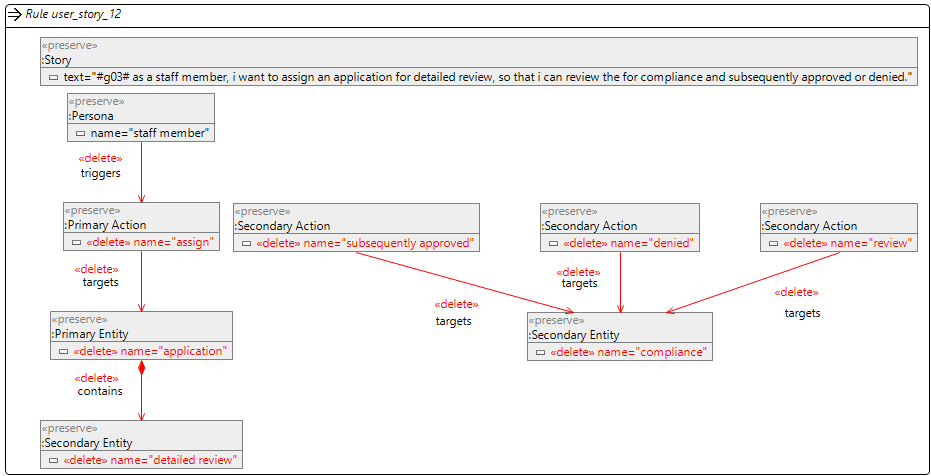
\includegraphics[scale=0.6]{rule_user_story_12}
%	\caption{Generated transformation rule related to user\_story\_12 using RuleCreator class}\label{fig:rule_user_story_12}
%\end{figure}
%As we can see, the "targets" edges and their direct relationships ("triggers" and "contain", if any) are also annotated as \textless delete\textgreater, which is very important to find redundant elements with the CDA tool.
%\end{example}
%\begin{example}
%Listing \ref{list:json_user_story_39} shows the JSON entities related to user\_story\_39 and Figure \ref{fig:rule_user_story_39} shows transformation rule generated by RuleCreator class.\\\\
%Text of US is:
%user\_story\_39: "\#G03\# As a Plan Review Staff member, I want to Review Plans, so that I can review them for compliance and either approve, or fail or deny the plans and record any conditions, clearances, or corrections needed from the Applicant."
%\begin{MyListing}
%	\paragraph{}
%	\centering
%	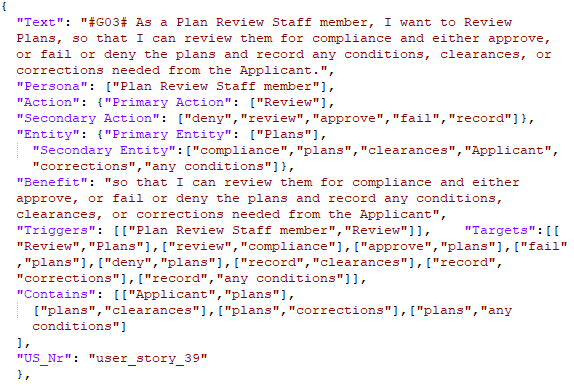
\includegraphics[scale=0.8]{Listing/json_user_story_39.png}
%	\caption{JSON entities Related to user\_story\_39}\label{list:json_user_story_39}
%\end{MyListing}
%\begin{figure}[h]
%	\centering
%	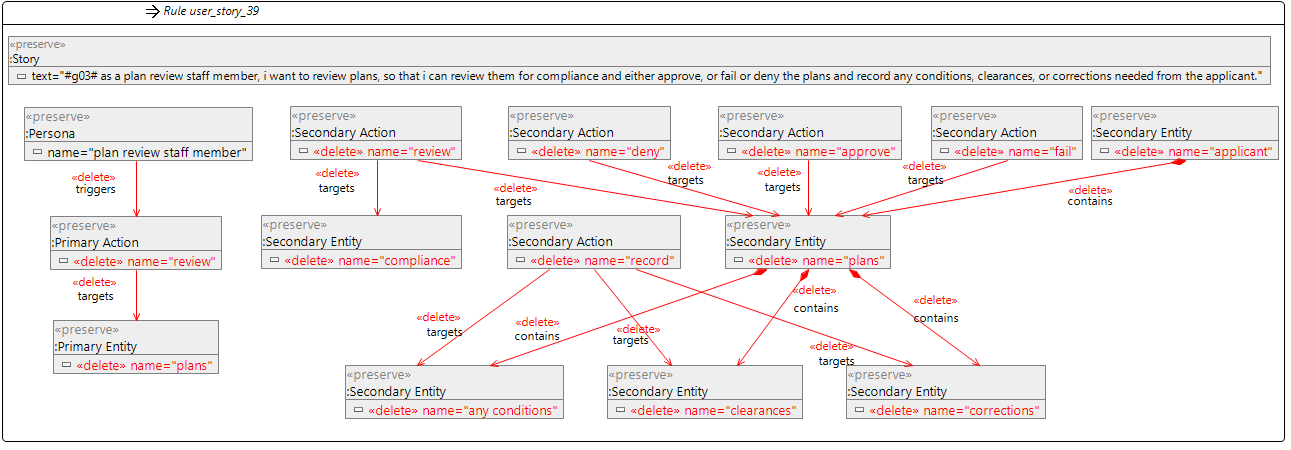
\includegraphics[scale=0.43]{rule_user_story_39}
%	\caption{Generated transformation rule related to user\_story\_39 using RuleCreator class}\label{fig:rule_user_story_39}
%\end{figure}
%Attribute "Plan", as we can see, it appears both in the main part as a primary entity and in the benefit part as a secondary entity, forming the various relationships as targets and contains.
%\end{example}

%\begin{example}
%Listing \ref{list:json_user_story_51} shows the JSON entities related to user\_story\_51 and Figure \ref{fig:rule_user_story_51} shows transformation rule generated by RuleCreator class.\\\\
%Text of US is:
%user\_story\_51: "\#G03\# As an Enforcement Staff member, I want to Issue a Notice of Violation, so that I can provide formal communication to the responsible party."
%\begin{MyListing}
%	\paragraph{}
%	\centering
%	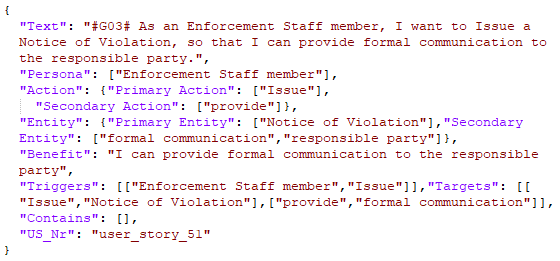
\includegraphics[scale=0.8]{Listing/json_user_story_51.png}
%	\caption{JSON entities Related to user\_story\_51}\label{list:json_user_story_51}
%\end{MyListing}
%\begin{figure}[h]
%	\centering
%	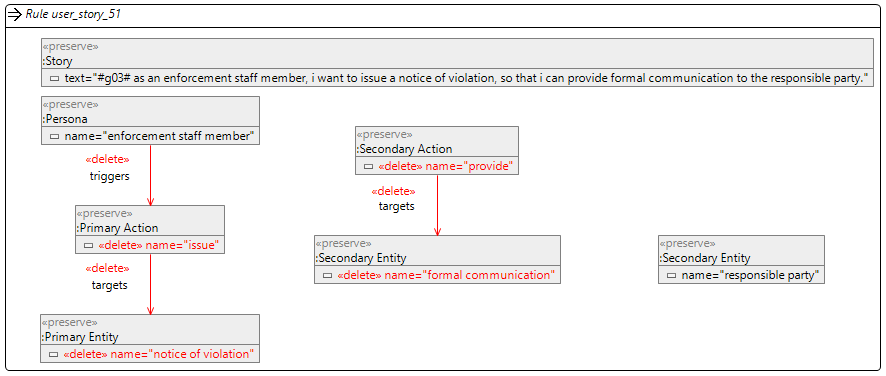
\includegraphics[scale=0.55]{rule_user_story_51}
%	\caption{Generated transformation rule related to user\_story\_51 using RuleCreator class}\label{fig:rule_user_story_51}
%\end{figure}
%Last but not least, we have determined that the secondary entity "responsible party" has neither a target nor a contains relationship. Therefore, it is not annotated as \textless delete\textgreater, but as \textless preserve\textgreater. This is due to the fact that some phrases have been identified as entities in the CRF tool, but their relationship is not annotated at all, which is problematic for analysing redundancy.
%\end{example}
\subsubsection*{Report Extraction}\label{step_report_extraction}
In order to extracting a textual report associated with a specific backlog, we implement a class called \textit{ReportExtractor} within the package \textit{org.henshin.backlog.code.report}, which include the following classes form the package \textit{org.eclipse.emf.ecore}\footnote{https://download.eclipse.org/modeling/emf/emf/javadoc/2.7.0/org/eclipse/emf/ecore/}. These classes are important for reading the content of minimal-model.ecore:
\begin{itemize}
	
	\item org.eclipse.emf.ecore.resource.Resource: A resource of an appropriate type is created by a resource factory; a resource set indirectly creates a resource using such a factory. A resource is typically contained by a resource set, along with related resources.
	
	\item org.eclipse.emf.ecore.resource.ResourceSet: A resource set manages a collection of related resources and notifies about changes to this collection. It provides a tree of content. A collection of adapter factories supports the search for an adapter via a registered adapter factory. 
	
	\item org.eclipse.emf.ecore.EObject: EObject is the root of all modelled objects, therefore all method names start with "E" to distinguish the EMF methods from the client methods. It provides support for the behaviour and functions that are common to all modelled objects.
	
	\item org.eclipse.emf.ecore.EPackage: A representation of the model object \enquote{EPackage}.
	
	\item org.eclipse.emf.ecore.EClassifier: A representation of the model object \enquote{EClassifier}.
	
	\item org.eclipse.emf.ecore.EClass: A representation of the model object \enquote{EClass}.
	
	\item org.eclipse.emf.ecore.EAttribute: A representation of the model object \enquote{EAttribute}.
	
	\item org.eclipse.emf.ecore.EReference:  A representation of the model object \enquote{EReference}.
	
\end{itemize}
\subsubsection*{Storing Redundancy Items into RedundancyItems Class}
To save the redundant elements found by the CDA tool, we implement classes to save the elements according to their type.

Figure \ref{fig:redundancyItems_class_diagram} is a class diagram that illustrates the attributes, operations and relationships related to the ReundancyItems class to store the redundancy elements provided by the CDA tool.
\begin{figure}[h]
	\centering 
	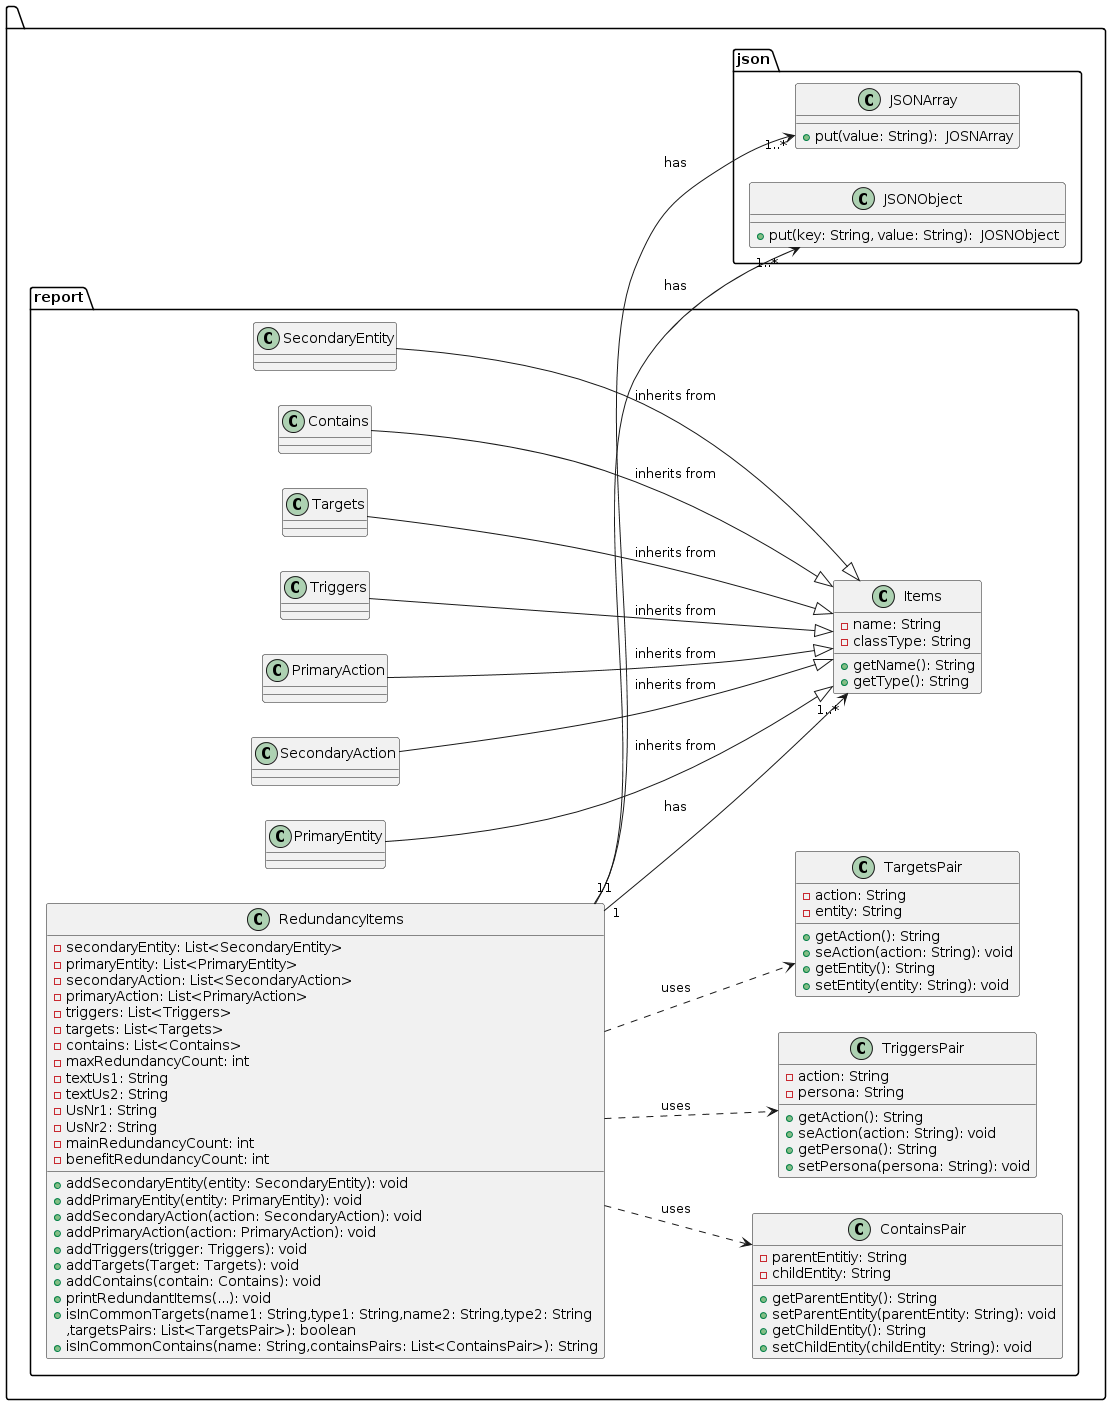
\includegraphics[scale=0.36]{redundancyItems_class_diagram.png}
	\caption{Class diagram for the RedundancyItems class and its relationship}\label{fig:redundancyItems_class_diagram}
\end{figure} 
The following classes were created to represent the extracted model object accordingly. All these classes are extensions of the class \textit{RedundancyItems}, which contains all extracted model object from \enquote{minimal-model.ecore} such as \enquote{EClass}, \enquote{EAttribute} or \enquote{EReference}:
\begin{itemize}
	
	\item PrimaryAction/SecondaryAction: Which has only saved the EClass specified by \enquote{Primary/Secondary Action} and the EAttribute model object with the methods \textit{getType} to retrieve the saved EClass and \textit{getName} to retrieve the saved EAttribute.
	
	\item PrimaryEntity/SecondaryEntity: Which has only saved the EClass specified by \enquote{Primary/Secondary Entity} and the EAttribute model object with the methods \textit{getType} to retrieve the saved EClass and \textit{getName} to retrieve the saved EAttribute.
	
	\item Targets: The EClass specified by \enquote{Primary/Secondary Action} as \textit{outgoing edge} and an EAttribute model object as \textit{incoming edge} with \enquote{Primary/Secondary Entity}. The method \textit{getType} retrieve the stored EClass and method \textit{getName} retrieve the stored EAttribute.
	
	\item Contains: The EClass specified by \enquote{Primary/Secondary Entity} as \textit{outgoing edge} and an EAttribute model object as \textit{incoming edge} with \enquote{Primary/Secondary Entity}. The method \textit{getType} retrieve the stored EClass and method \textit{getName} retrieve the stored EAttribute.
	
	\item Triggers: The EClass specified by \enquote{Persona} as \textit{outgoing edge} and an EAttribute model object as \textit{incoming edge} with \enquote{Primary Action}. The method \textit{getType} retrieve the stored EClass and method \textit{getName} retrieve the stored EAttribute.
	
	\item RedundantPair: Stores the identifier of the two USs that were founded as a redundant pair. It also stored the total count of redundancy clauses within the US-pair.
	
	\item TargetsPair: Stores effective value of \enquote{\textit{Primary/Secondary Action}} and \enquote{\textit{Primary/Secondary Entity}} in action and entity fields accordingly.
	
	\item ContainsPair: Stores effective value of \enquote{\textit{Primary/Secondary Entity}} as \enquote{\textit{parent/child entity}} due to the fact that parent entity is a containment of child entity.
	
	\item TriggersPair: Stores effective value of \enquote{\textit{Persona}} as a persona and \enquote{\textit{Primary Action}} as an action.
	
\end{itemize}
The class RedundancyItems contains following methods which are important for class ReportExtractor:
\begin{itemize}
	\item isInCommonContains: This method is designed to determine whether a given entity (specified by its name) is part of a redundant pair listed in the \enquote{Contains} array of related USs stored in a JSON file.
	
	As input, it receives the name of the entity for which we want to Checks whether it exists in a redundant pair. In addition, a list of redundant pair objects that represent pairs of entities where one entity contains the other. If there is a match with the parent entity, it returns the child entity and vice versa.
	\item isInCommonTargets: This method is responsible for determining whether a particular action/entity is part of a redundant pair listed in the "Targets" array of related USs stored in a JSON file.
	
	As input, it receives the name and type of the first element, which is an action, and the name and type of the second element, which is an entity. It also receives a list of TargetsPair objects, which are pairs of common actions and entities between US-pairs.
	
	For each pair, it checks whether the specified names and types match either the action or entity in the pair. If a match is found, the method returns \textit{true}, which means that the specified elements are part of a redundant pair.
	\item printRedundantItems: This method is responsible for creating a report on redundancy items based on the data stored in the class instance. 
	
	As input, it takes several parameters, including a "FileWriter" to write to the textual report's file, lists of different pairs of "Targets", "Contains" and "Triggers", and a JSON-object to store the report data in JSON format, which is vital for evaluation.
\end{itemize}
\subsubsection*{ReportExtractor Class: Methods related to Extracting Redundancy Items}
To extract the redundant elements and save them in a redundancyItems object, we must first iterate through all existing \textit{minimal-mode.ecore} files and extract the redundant reduandcy item from each EPackage.

Figure \ref{fig:report_extractor_class_diagram} is a class diagram that illustrates the attributes, operations and relationship related to the extraction of redundancy items founded by the CDA tool and their storage in a RedundancyItems object.
\begin{figure}[h]
	\centering
	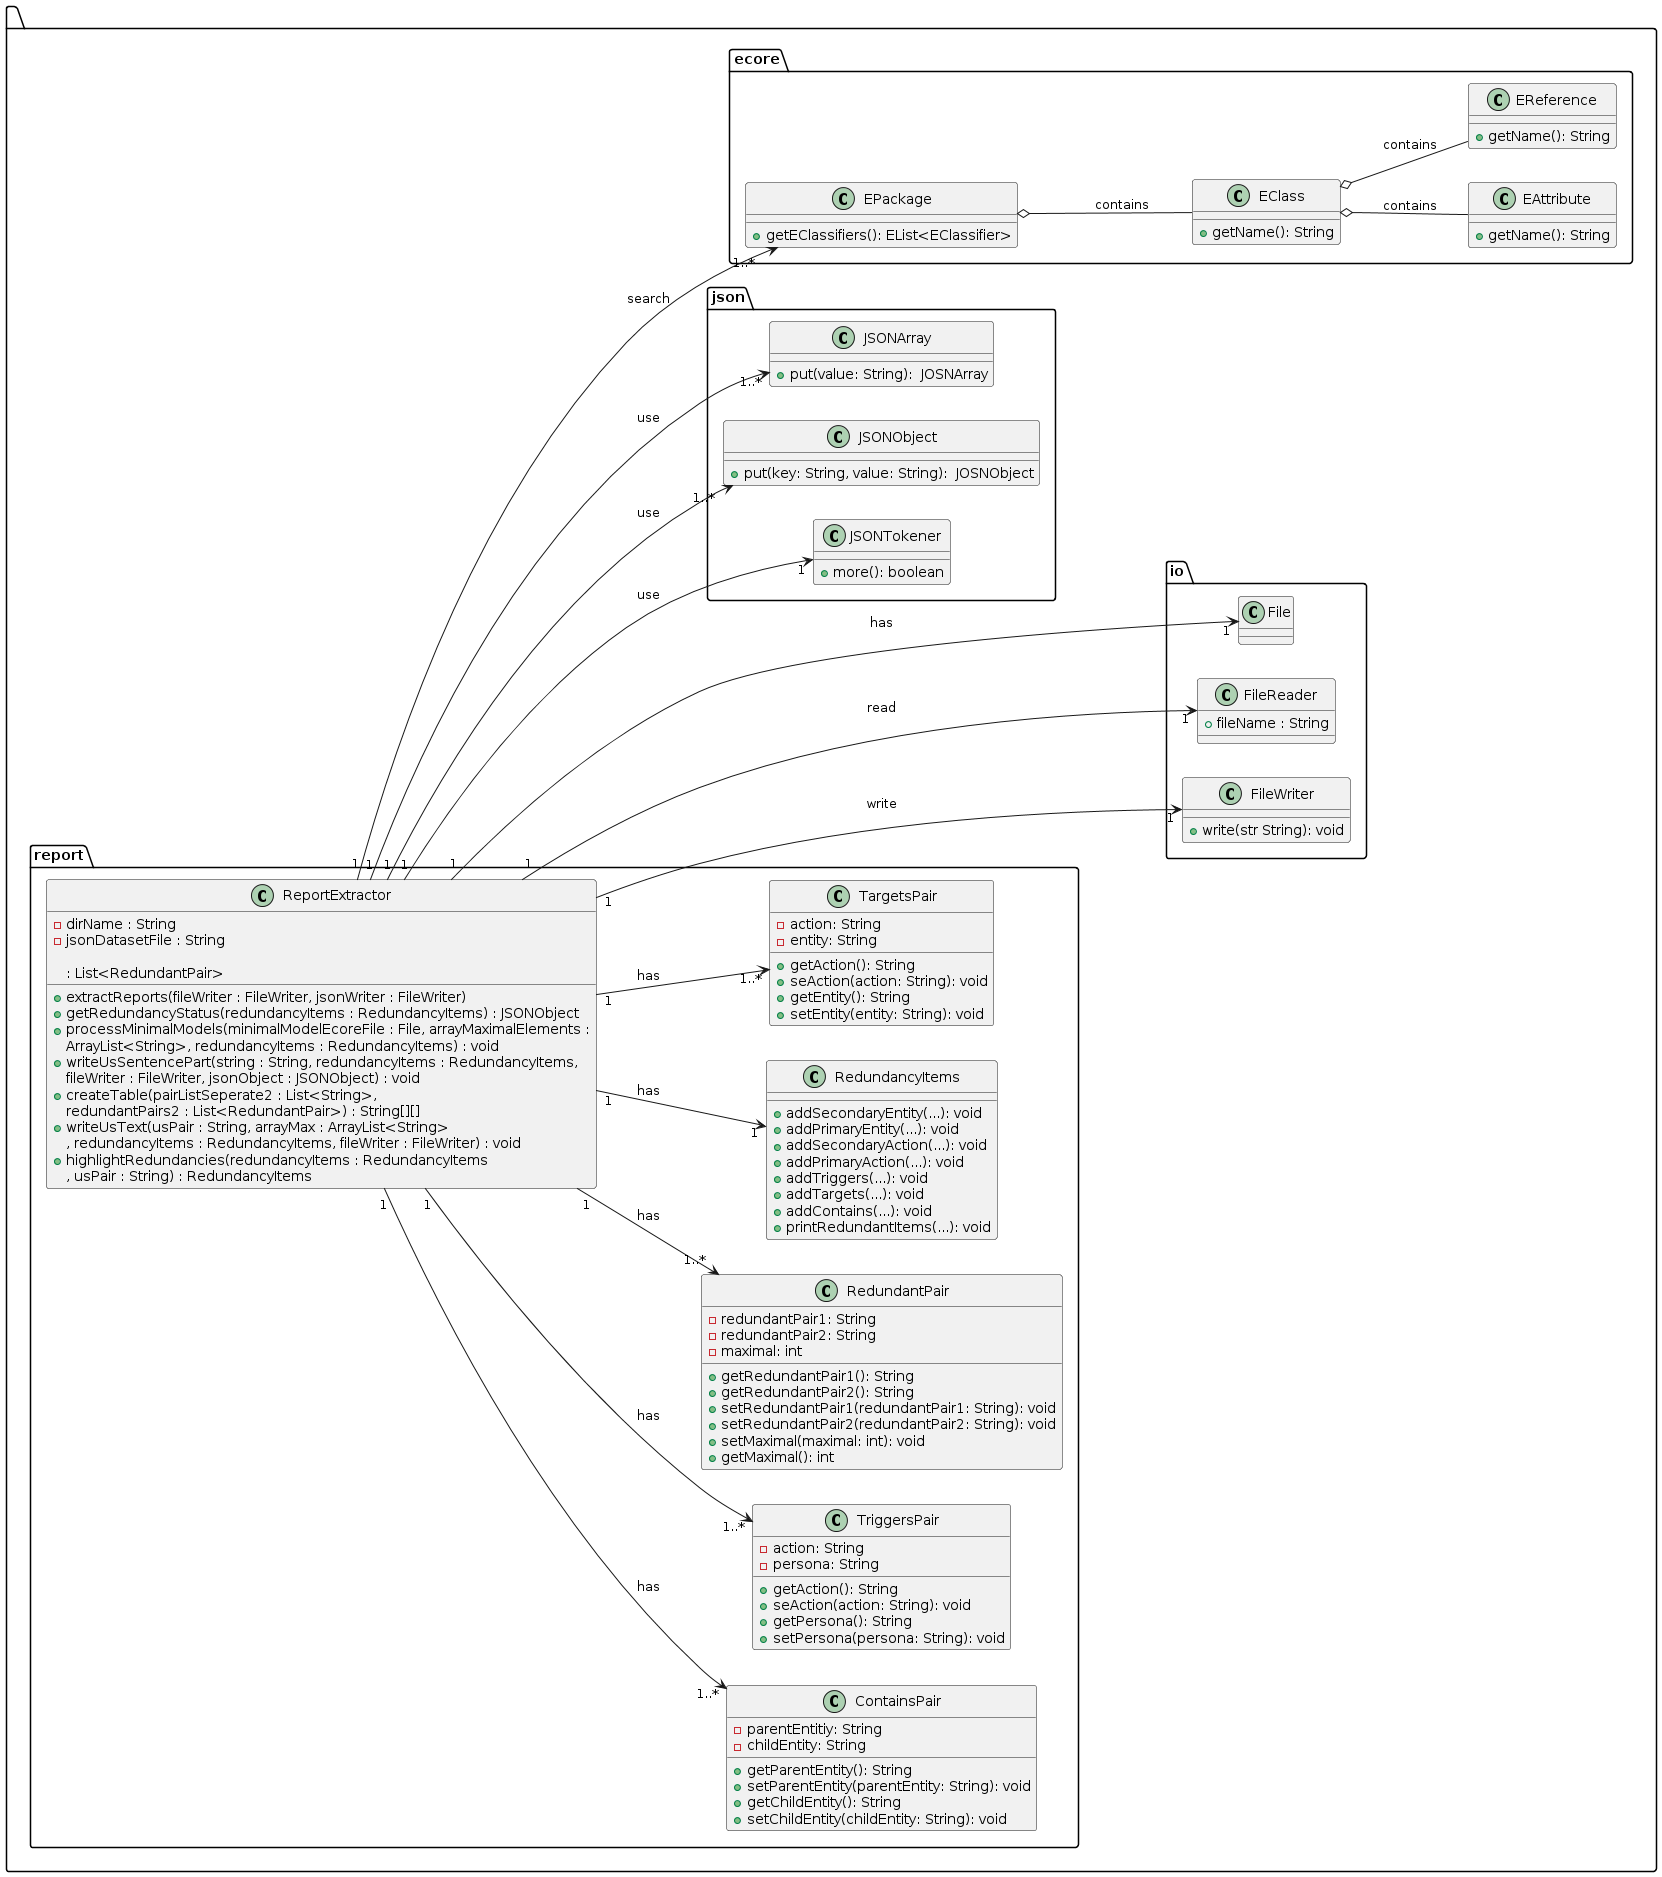
\includegraphics[scale=0.27]{report_extractor_class_diagram}
	\caption{Class diagram for the process of extracting redundancy items}\label{fig:report_extractor_class_diagram}
\end{figure} 

The following methods in the ReprortExtractor class are responsible for extracting the redundancies found by the CDA tool:
\begin{itemize}
	\item extractReports: This method orchestrates the extraction and analysis of created CDA report from a directory containing conflicted US-pairs and their associated reasons(conflict reason), and generates both text and JSON reports for further investigation and processing.
	
	It receives two FileWriter objects as input, one for writing textual and one for JSON reports.
	
	It iterates through each directory in the main directory that represents a conflict pair and uses the \textit{checkIfReportExist} method to make sure that the current US-pair are not already proceeded and the \textit{containsAnd} method to Checks whether it contains the conjunction \enquote{AND} to make sure that it is the valid US-pair name(\textit{e.g.} "user\_stroy\_12\_AND\_user\_stroy\_39" is a valid directory name).
	
	For each valid conflict pair directory, it iterates through the conflict reason directories within the current conflict pair directory and uses the \textit{minimalEcoreExist} method to Checks whether a \textit{minimal-model.ecore} file exists with reference to a conflict reason.
	
	To identify redundancy items, it uses the method \textit{processMinimalModels} and reads the "minimal-model.ecore" file, processes its content and iterates over the contained EPackages in order to process them further with the method \textit{iteratePackages}, which saves all redundancy items in RedundacyItems object.
	
	In addition, the methods \textit{hasEntitys}, \textit{hasActions} and \textit{hasTargets} are used to Checks whether the identified elements contain "Primary/Secondary actions" and "Primary/Secondary Entities" with common "Targets" reference. If the identified elements fulfil the criteria, the redundancy pair is included in the report.
	
	It then writes the potentially redundant USs and their clauses to the textual as well as JSON report files for further analysis.
	
	As output, the method returns a list of RedundantPair objects containing information about identified redundancies between US-pairs.
	
	\item createOrOverwriteReportFile: The method is responsible for creating or overwriting report file. It first ensures the existence of a report file. If the file doesn't exist, it creates a new one; if it already exists, it overwrites the existing file. Finally, it returns a \textit{FileWriter} to allow writing to the report file.
	
	\item checkIfReportExist: This method takes two parameters, namely US-pair and the list of all previously processed pairs in the CDA report directory. It returns \textit{true} if the US-pair was found in the pairList, which means that a report with the specified pairs has already been executed and therefore does not need to be executed again.
	
	\item minimalEcoreExist: This method checks the existence of a \textit{minimal-model.ecore} file using a conflict pair and a conflict reason generated by CDA tool.
	
	As input, it receives a conflict pair and a conflict reason. Using these parameters, the method constructs the file path to the minimal-model.ecore file and checks whether the file exists under the constructed path.
	
	If the ECore file exists, the method returns \textit{true}, indicating that the minimal-model.ecore file exists for the examined conflict pair and conflict reason. If the file does not exist, \textit{false} is returned.
	
	\item containsAnd: This method ensures that the folder name is identified with "\textit{\_AND\_}", as the report generated by CDA tool is formatted like \enquote{user\_story\_\textless digit \textgreater \_AND\_ user\_story\textless digit \textgreater}. It returns \textit{true} if the examined directory contains \enquote{AND}, otherwise \textit{false} is returned.
	
	\item processMinimalModels: This method reads a Minimal Model Ecore file, processes its content and iterates over the contained EPackages in order to process them further with the \textit{iteratePackages} method. 
	
	As parameters, it receives a File object that represents examined minimal model ecore file, an array list in which the names of the redundant elements are stored, and a RedundancyItems object that is used to handle redundant elements. 
	
	First, a ResourceSet and a ResourceFactoryRegistry corresponding to the minimal model Ecore file are set up and a Resource object is created from the Ecore file; the \textit{iteratePackages} method is called for each EPackage.
	
	\item iteratePackages: This method identifies redundancies within the attributes and references of EClasses in examined minimal model, stored them accordingly and updates the RedundancyItems object.
	
	It takes several parameters, such as the EPackage to be iterated over, an array list in which the names of the redundant elements are stored, and a RedundancyItems object. 
	
	It iterates through every EClassifier in the minimal package that contains EClasses and checks whether \enquote{\#} is present in EClass; if this is the case, EClass has been recognised as a conflict by CDA tool.
	
	If an attribute is found, the class of the conflicting attribute is determined and added to the corresponding element within RedundancyItems (e.g. Primary/Secondary Action/Entity). 
	
	Each EReference is then iterate through in the EClass. Depending on the reference name, the reference is added to the corresponding element within RedundancyItems (e.g. Triggers, Targets, Contains). The method is completed once all EClassifiers within the specified EPackage have been processed.
	
	\item hasActions: This method is useful for using the data stored in RedundancyItem to determine whether certain actions are present in a list of redundant entries, in order to later Checks whether the identified elements fulfil the criteria and the redundancy pair is included in the report.
	
	It checks if there's a match with name of any primary/secondary action stored in the RedundancyItems object. If match is found, it immediately returns \textit{true}.
	
	\item hasEntitys: This method is used to determine whether certain secondary/primary entities  are present in the RedundancyItems object based on their name. For each item, it checks whether there is a match with the name of a primary/secondary entity stored in the RedundancyItems object. 
	
	If a match is found, \textit{true} is returned immediately, in order to later Checks whether the identified elements fulfil the criteria and the redundancy pair is included in the report.
	
	\item hasTargets: This method uses the content of a RedundancyItems object to determine whether targets are present in a list of founded redundant elements.
	
	As input, it receives an array list with the names of the redundant elements and an object of the type RedundancyItems, which contains a collection of founded "Targets".
	
	The method checks whether there is a match with the name of any targets reference stored in the RedundancyItems object. 
	
	If a match is found between the elements, the method immediately returns \textit{true}, which means that at least one targets reference is present, in order to later Checks whether the identified elements fulfil the criteria and the redundancy pair is included in the report.
	
	\item readJsonArrayFromFile: This method provides the ability to read JSON data from a file and convert it into a JSONArray object, handling cases where the file is empty or does not exist.
	
	It receives the file path of the JSON file to be read as input. An attempt is made to open the specified file and Checks whether the file is empty or does not exist. If the file exists and is not empty, it reads the JSON data from the file and creates a JSON array object from the JSON data read from the file and returns the JSON array object with the JSON data.
	
	
	\item getRedundancyStatus: This method add statistics like count of main/benefit/total redundancies into JSON report. It receive as input redundancyItems and as output write the count of main/benefit/total redundancies into JSON report already defined in method highlightRedundancies.
\end{itemize}
\subsubsection*{Methods for Extracting Data from Dataset of Backlog}
To get information about USs such as text, redundant clauses in targets/contains/triggers references between US-pairs, we need to extract data from the dataset stored in the JSON file.
%Figure \ref{fig:json_data_extractor_diagram} illustrate the communication between three processes.
%\begin{figure}[h]
%\centering 
%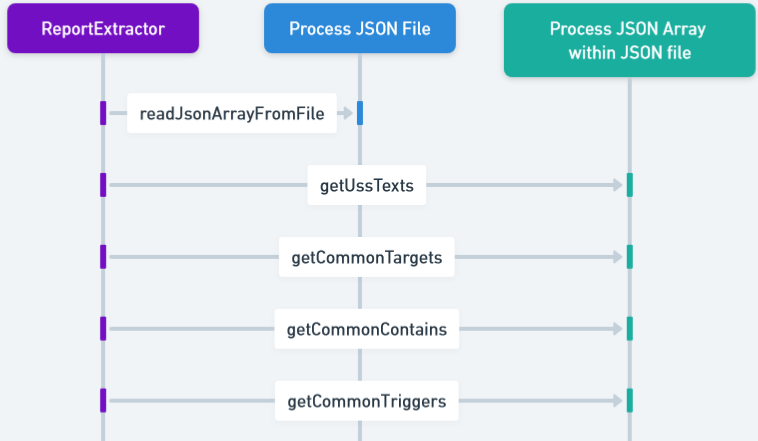
\includegraphics[scale=0.35]{data_extractor_diagram}
%\caption{Sequence diagram for the processes of extracting common entries between two USs from dataset of the %backlog}\label{fig:json_data_extractor_diagram}
%\end{figure} 

The following methods in the ReprortExtractor class are responsible for extracting data from dataset within JSON file:
\begin{itemize}
	\item readJsonArrayFromFile: This method receives a JSON file as input. After reading, the JSON content is tokenised, parsed into a JSON array and the parsed JSON array is returned.
	
	\item getUssTexts: This method ensures that the text of the specified US-pair is retrieved from the JSON file and properly assigned to the RedundancyItems object for further processing. It receives a US-pair and RedundancyItems as input. 
	
	It reads a JSON array from a file using the \textit{readJsonArrayFromFile} method, iterates over each JSON object in the array and compares the extracted US identifier with the US identifier extracted from the input US-pair. If a match is found, the text of the first and second USs is set in the redundancyItems object.
	
	\item getCommonTargets: Used to determine overlaps in "Targets" references (pairs of actions and entities) between specified US-pairs from a JSON file.
	
	It receives the identifiers of the US-pair as input. After it finds the US objects, it compares each pair of entries (actions and entities) in "Targets" references of the two USs and looks for matches.
	
	The output is the matches, i.e. the list of common pairs of actions and entities, in "Targets" reference.
	
	\item getCommonContains: Used to determine overlaps in "Contains" references (pairs of entities) between specified US-pairs from a JSON file.
	
	It receives the identifiers of the US-pair as input. After it finds the US objects, it compares each pair of entities in "Contains" references of the two USs and looks for matches.
	
	The output is the matches, i.e. the list of common pairs of entities, in "Contains" reference.
	
	\item getCommonTriggers: Used to determine overlaps in "Triggers" references (pairs of personas and actions) between specified US-pairs from a JSON file.
	
	It receives the identifiers of the US-pair as input. After it finds the US objects, it compares each pair of entries (personas and actions) in "Triggers" references of the two USs and looks for matches.
	
	The output is the matches, i.e. the list of common pairs of personas and actions, in "Triggers" reference.
\end{itemize}
\subsubsection*{Methods for Highlighting Words using Hash Symbol(\#)}
In order to distinguish redundancy words between a US-pair, in text of each US, we decide to highlighting redundant words using hash symbol like \enquote{ ... \#\textless word\textgreater\# ... }.
%Figure \ref{fig:highlight_diagram} is a sequence diagram that illustrates the communication between processes related to the highlighting of redundancy words.
%\begin{figure}[h]
%\centering 
%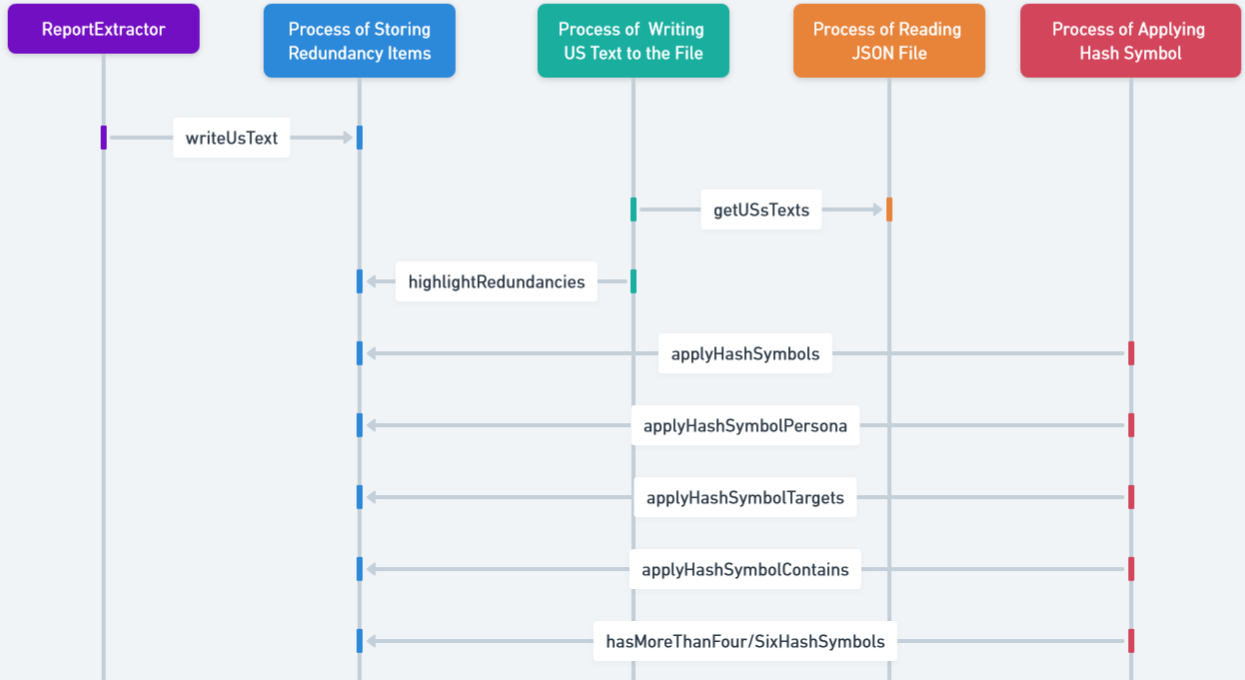
\includegraphics[scale=0.35]{highlight_diagram}
%\caption{Sequence diagram for the process of highlighting redundancy clauses in the Texts of US-pair}\label{fig:highlight_diagram}
%\end{figure} 

The following methods in the ReprortExtractor class are responsible for highlighting redundancy words:
\begin{itemize}
	\item writeUsText: This method reads the text of examined US-pair, highlights redundant element between them using \textit{highlightRedundancies} method, writes the highlighted text to a file, and records information about the redundant elements. 
	
	As input it receive a US-pair, a list of redundant pairs to store redundant pairs in it, an object RedundancyItems containing stored redundancy elements and a FileWriter object used for writing output.
	
	It extract the identifier of the two USs from US-pair, retrieves the text of the USs from JSON file and add them to RedundancyItems, invoke the \textit{highlightRedundancies} method to identify and highlight redundants between the USs, it writes the highlighted text of each US to the FileWriter. Finally, sets the redundant pair and count of redundancy clauses.
	\item highlightRedundancies: This method identifies redundancies between US-pair, applies hash symbols using \textit{applyHashSymbols} method to highlight common items and updates the redundancy counts in the redundancyItems object. 
	
	It takes two parameters, redundancyItems and US-pair, which represents the pair of USs to be analysed. 
	
	It checks whether both USs contain a main clause part or whether one of them has a benefit part or whether both USs also have a benefit part.
	
	It applies hash symbols to common elements that only occur in the part of the USs that occurs in the same part (e.g. only main or only benefit part of the USs). 
	
	In each condition, it checks if there are redundancy clauses in the main part, then persona is also highlighted using \textit{applyHashSymbolPersona} method. It also updates the count of main/benefit/total redundancies and sets the changed text of USs. Finally, it returns the updated redundancyItems object.
	\item applyHashSymbols: This method is used to mark certain words within a substring with hash symbols (\#) at the beginning and end to ensure that they are distinguishable and can be easily identified or processed later. 
	
	It takes a substring in which replacements are to be made and a field of matches containing the words to be surrounded with hash symbols. First, the field of matches is sorted in descending order of length and processed accordingly to avoid adding hash symbols to unwanted clauses. 
	\begin{example}
		For example, let's assume that we have \enquote{data} and \enquote{data format} as redundancy elements. If we continue first with \enquote{data} and then with \enquote{import data}, \enquote{import data} will be replaced by \enquote{import \#data\#}, which is not desired.
	\end{example}
	\item hasMoreThanFour/SixHashSymbols: These methods receive a text from the US as input. They are used to Checks whether there are redundant clauses in the main part of the sentence (it can be one or two clauses). If so, \textit{true} is returned.
	
	\item applyHashSymbolPersona: This method identifies common "Triggers" references, marks them with hash symbols and returns the changed text parts together with the count of redundant triggers references. 
	
	As input, it receives a list of common triggers between US-pair, RedundancyItems and the parts of the USs. It iterates through the list of common triggers and checks whether both elements(persona and primary action) of the triggers are present in both parts. 
	
	It then increments the redundancy count to keep track of the count of redundant triggers. The output returned, is the text of USs containing the manipulated text parts with hash symbols and the redundancy count in main part.
	
	\item applyHashSymbolTargets: This method identifies common targets references between two parts of USs, marks them with hash symbols and returns the changed text parts together with the count of redundant targets references.
	
	As input, it receives a list of common targets between the US-pair, RedundancyItems and the parts of the USs. 
	
	It iterates through the list of common targets and checks whether both elements (primary/secondary action and primary/secondary entity) of the targets are present. It then increments the redundancy count in examined part of USs to keep track of the count of redundant targets. 
	
	The output returned is the text of USs containing the manipulated text parts with hash symbols and the redundancy count in examined part(main or benefit).
	
	\item applyHashSymbolContaians: This method identifies common contains references between two parts of USs, marks them with hash symbols and returns the changed text parts together with the count of redundant contains references. 
	
	As input, it receives a list of common contains between the US-pair, RedundancyItems and the parts of the USs. It iterates through the list of common contains and checks whether both elements of the contains are present in both parts. It then increments the redundancy count to keep track of the count of redundant contains.
	
	The output returned is the text of USs containing the manipulated text parts with hash symbols and the redundancy count in examined part(main or benefit).
	
\end{itemize}
\subsubsection*{Methods related to Report Divided Parts of USs}
To show which part of the USs with redundancy words occur between a US-pair, we have split the individual parts of the USs and included them in the report.
%Figure \ref{fig:splitUsText_diagram} is a sequence diagram that illustrates the communication between processes related to the splitting of parts of a US-pair containing redundancy words.
%\begin{figure}[h]
%\centering 
%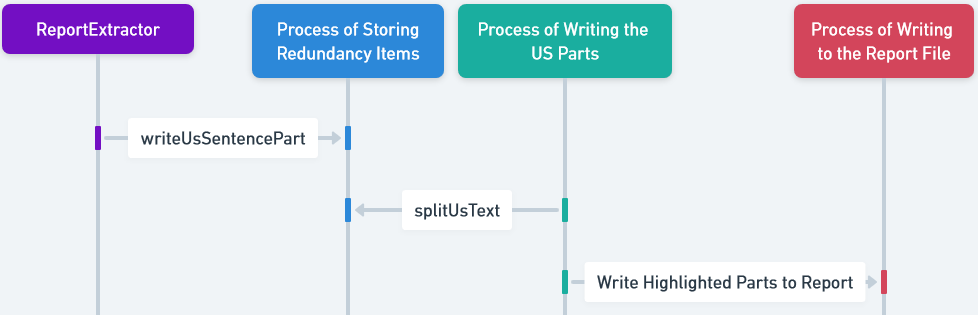
\includegraphics[scale=0.35]{splitUsText_diagram}
%\caption{Sequence diagram for the process of splitting parts of US-pair containing redundancy word}\label{fig:splitUsText_diagram}
%\end{figure} 
The following methods in the ReprortExtractor class are responsible for splitting and reporting the parts of the USs :
\begin{itemize}
	
	\item splitUsText: This method is used to split the text of two USs into separate sections based on the occurrence of redundancy clauses. 
	
	The input is the text of the first and second US and their corresponding identifiers, a FileWriter for writing to a file and a JSON object for processing JSON data. 
	
	It splits each US text into three parts using commas and saves the result in arrays. It iterates over parts of the first and second USs and searches for occurrences of hash symbol pairs. For each part, the number of hash symbol pairs found is counted. Finally, all parts of the records that contain hash symbols are written to a text file and a JSON file as well.
	
	\item writeUsSentencePart: This method facilitates the extraction and storage of highlighted USs parts from US-pair in a textual report file for further analysis.
	
	As input, it receives the US-pair, RedundancyItems and a FileWriter allowing the extracted USs parts to be written. It receives the text of the USs from the reundancyItems object and calls the \textit{splitUsText} method to split the US-pair texts into USs parts with highlighted elements.
	
	The extracted USs parts are also written to the text and JSON report files, using the FileWriter for further processing and analysis.
	
	\begin{example}
		Take, for example, the following US-pair:
		
		\textit{user\_story\_60:} \#g22\# as an it staff member, I want to \#know\# \#how\# the \#data\# is \#used\#, so that I can determine what kind of basic services and functionalities are required.\\\\
		\textit{user\_story\_04:} \#g22\# as a data manager, I want to \#know\# \#how\# the \#data\# is \#used\#, so that I can develop more detailed usage and support scenarios with researchers.\\\\
		The following sentence parts are candidates for possible redundancies between user stories:\\\\
		user\_story\_04:  I want to \#know\# \#how\# the \#data\# is \#used\#\\\\
		user\_story\_60:  I want to \#know\# \#how\# the \#data\# is \#used\#	
	\end{example}
\end{itemize}
\subsubsection*{Methods related to Creating Table}
The summary of potential redundancy between US-pairs is presented in a table, which makes it easy to find out which US-pairs have been identified as potentially redundant US-pairs and how many redundancy elements there are in total.
%Figure \ref{fig:writeTable_diagram} is a sequence diagram that illustrates the communication between the processes related to creating tables and addition to text reports.
%\begin{figure}[h]
%\centering 
%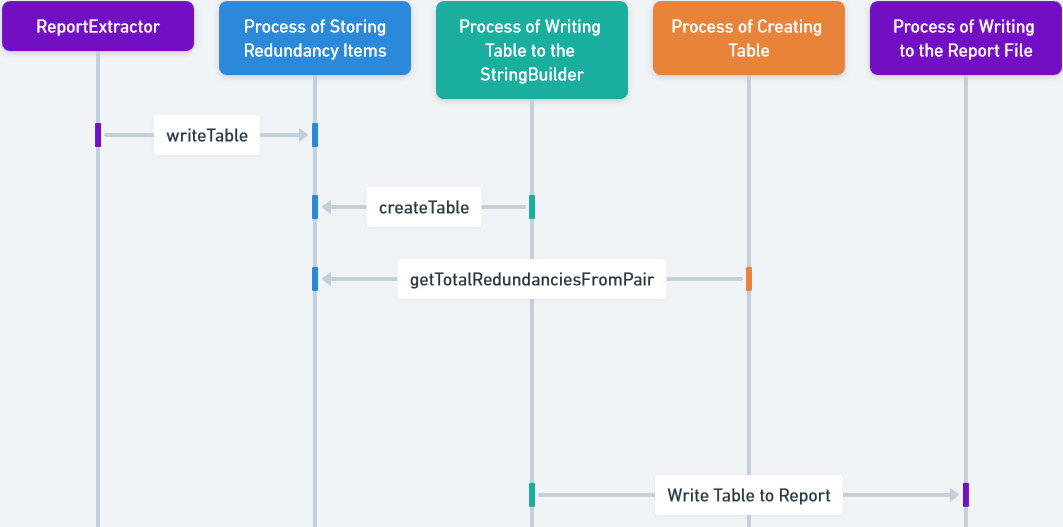
\includegraphics[scale=0.35]{writeTable_diagram}
%\caption{Sequence diagram for the process of creating and adding tables to the textual report}\label{fig:writeTable_diagram}
%\end{figure} 
The following methods in the ReprortExtractor class are responsible for creating a table at the beginning of the text report:
\begin{itemize}
	\item writeTable: This method is used to write a table of potential redundancies between USs and the count of their total redundant clauses \textit{createTable} method.%, including the addition of the count of main and benefit redundancy clauses using \textit{createTable} method.
	
	As input, it receives a File object into which the table is inserted and a list of redundancy pairs containing information about redundant clauses in US-pars.
	
	It reads the existing content of the textual report file into a StringBuilder. It creates a table to display the potential redundancies between USs and the count of total redundancy clauses.
	
	The table headers and contents are generated based on the redundant pairs. It calculates the maximum width for each column in the table to ensure proper formatting. Finally, the table content is written to the FileWriter, followed by the existing content stored in the report's StringBuilder.
	
	\item createTable: This method prepares the content for the table in which potential redundancies between USs are displayed, taking into account the total redundancy count between each US-pairs based on the RedundantPair objects provided.
	
	As input, it receives a list of unique US-pairs for which the table is to be created and a list of RedundantPair objects containing information about redundant clauses between US-pairs.
	
	It initialises a two-dimensional array containing the contents of the table. The size of the table is determined by the count of unique pairs of USs plus one for the header row and column.
	
	It fills the header row and the first column of the table with unique pairs of US-pairs, replacing \enquote{user\_story} with \enquote{us} for the purpose of brevity.
	
	It calculates the maximum redundancy count between each US-pair by calling the method \textit{getTotalRedundanciesFromPair}. Finally, it fills the table with the total redundancy count. 
	
	The output is a two-dimensional array representing the contents of the table, with each cell containing the maximum redundancy count between the corresponding pair of USs.
	
	\item getTotalRedundanciesFromPair: This method makes it easier to retrieve the total number of redundancies between a US-pair from a list of RedundantPair objects.
	
	As input, it receives a list of RedundantPair objects containing information about redundant elements in US-pairs, where the first and second USs are to be compared.
	
	It iterates through each RedundantPair object in the RedundantPairs list and checks for each RedundantPair object whether the examined US-pair matches as redundant US-pair. 
	
	If a matching pair is found, the maximum redundancy number stored in this RedundantPair object is returned. If no matching pair is found, \textit{zero} is returned, indicating that there are no redundancies between the examined US-pair.
\end{itemize}
\subsubsection*{Report Evaluation}\label{step_report_evaluation}
The Evaluation class, found in the \textit{org.henshin.backlog.code.evaluation} package, was created to assess redundancy levels in USs based on JSON reports. This class includes methods that evaluate whether two USs are fully or partially redundant, focusing on various application components within these USs.

Figure \ref{fig:evaluation_class_diagram} is a class diagram that illustrates the attributes, operations of the Evaluation class and its relationship to other classes.
\begin{figure}[h]
	\centering 
	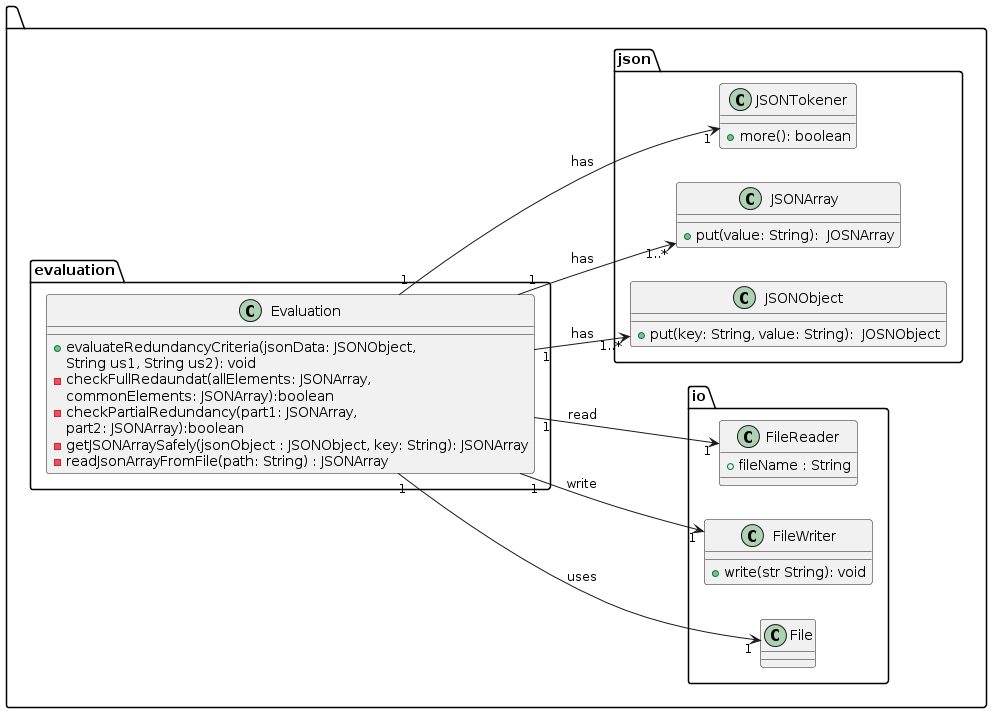
\includegraphics[scale=0.4]{evaluation_class_diagram}
	\caption{Class diagram related to Evaluation class}\label{fig:evaluation_class_diagram}
\end{figure} 
The class offers a detailed mechanism to evaluate redundancy through following methods:
\begin{itemize}
	\item\textit{evaluateRedundancyCriteria}: This method compares elements such as "Triggers", "Targets" and "Contains" in the "Main" and "Benefit" parts of USs. The method checks whether these clauses are fully redundant (i.e. they are identical between USs) or partially redundant (i.e. they share some clauses but are not fully identical).
	
	As input, it receives the JSON object for a specific US-pair.
	
	In particular, it checks various conditions, e.g. whether common clauses are present, whether targets or contains are empty and whether the clauses in the stories are fully or partially identical.
	
	As output, the method updates the JSON report with new keys indicating the redundancy status:
	
	Main Part Fully Redundant: A Boolean value indicating whether the "main part" of the USs is fully redundant.
	
	Main Part Partially Redundant: A Boolean value that indicates whether the "main part" of the USs is partially redundant.
	
	Benefit Part Fully Redundant: A Boolean value that indicates whether the "benefit part" of the USs is fully redundant.
	
	Benefit Partially Redundant: A Boolean value that indicates whether the "benefit part" of the USs is partially redundant.
	
	\item checkPartialRedundancy: The method processes these arrays to identify partial redundancy by checking whether elements from arrays of elements match elements from another array. 
	
	It receives the two arrays of elements as input, iterates through each element of the first input array and compares each of these elements with all elements in the second input array. A match counter records how often elements from the first input array find a match in the second input array.
	
	As output, method returns a Boolean value. True: indicates that there is at least one matching element pair between the two JSON arrays, which means partial redundancy. False: indicates that there are no matching elements, indicating no partial redundancy between these specific parts of the USs.
	
	\begin{example} Assume we have the following JSON arrays for two different USs: \\\\
		First JSON array: [["login", "button"], ["help", "link"]]\\
		Second JSON array:	[["logout", "button"], ["help", "link"]]\\\\
		The method would determine that the second element of the first array ("help", "link") matches the second element of the second array. As there is at least one match, checkPartialRedundancy would return true, indicating partial redundancy.
	\end{example}
	
	
	\item getJSONArraySafely: This method is designed to handle JSON operations safely by retrieving JSON array from a JSON object without the risk of throwing exceptions if the specified key does not exist.
	
	As input it receives the JSON object from which the JSON array needs to be extracted and a key corresponding to the JSON array within the provided JSON object.
	
	The method first checks whether the provided key exists in the JSON object. If the key exists, it retrieves the JSON array associated with that key. If the key does not exist, it returns an empty JSON array.
	\begin{example} Let's assume that a JSON object representing USs details should contain the key for "Benefit Part", which does not exist:\\
		\{\\
		"Common Targets" : \{\\
		"Main Part" : [["login","button"],["help","link"]]
		\}\\
		\} \\\\
		If the "Benefit Part" in the "Common Targets" needs to be accessed that does not exist, this is handled safely with \textit{getJSONArraySafely} by returning an empty array to avoid runtime errors.
	\end{example}
	
	\item readJsonArrayFromFile: The method enables JSON data to be read from a file and converted into a JSON array object. It takes the file path as input and attempts to open the file, checking whether the file is empty or missing. If the file is available and contains data, this data is read, converted into a JSON array object and returned.
	
\end{itemize}
\subsubsection*{Error Handling}
There were erroneous data in datasets that force us to handle them correctly. Therefore, we implement/use the following exceptions to accurately distinguish and handle them.

The following classes, which extend the \textit{Exception} class, are used in the \textit{org.henshin .backlog.code.rule} package and relate to error handling related to the JSON entries in the dataset of the backlogs and to the Ecore meta-model required to create the rules based on it:
\begin{itemize}
	\item EmptyOrNotExistJsonFile: Is triggered if the JSON file could not be found in the file system.
	
	\item ActionInJsonFileNotFound: Is triggered if the entry \textit{Action}, which contains \textit{Primary/Secondary Actions}, is not present in the JSON file and its absence should be reported.
	
	\item EntityInJsonFileNotFound: Is triggered if the entry \textit{Entity}, which contains \textit{Primary/Secondary Entity}, is not present in the JSON file and its absence should be reported.
	
	\item PersonaInJsonFileNotFound: Is triggered if the entry \textit{Persona} does not exist in the JSON file for a specific US.
	
	\item TextInJsonFileNotFound: Is triggered if the entry \textit{Text} does not exist in the JSON file for a specific US. 
	
	\item UsNrInJsonFileNotFound: Is triggered if the entry \textit{Us\_Nr} does not exist in the JSON file for a specific US.

	\item EdgeWithSameSourceAndTarget: Refers to the creation of edges in graph transformation rules and is triggered if the source and target of the edge have already been created, then the duplicate edge should be avoided.
		
	\item TargetsInJsonFileNotFound: Is triggered if the entry \textit{Targets} does not exist in the JSON file for a specific US.
	
	\item ContainsInJsonFileNotFound: Is triggered if the entry in \textit{Contains} is not present as \textit{Primary/Secondary Entity} in the JSON file and its absence should be reported.
	
	\item TriggersInJsonFileNotFound: Is triggered if the entry \textit{Triggers} does not exist in the JSON file for a specific US. 
	
	\item EcoreFileNotFound: Is triggered if the required ECore meta-model file could not be found and should also be reported.
\end{itemize}
Within the \textit{org.henshin.backlog.code.report} package, special classes that extend the \textit{Exception} class are designed to solve problems related to the CDA report directory, which encapsulates all US-pairs together with the associated conflict reasons. These classes include:
\begin{itemize}
	\item CdaReportDirIsEmpty: This exception is called if the CDA report directory is found but has no content.
	\item CdaReportDirIsNotADirectory: This exception is thrown in scenarios where the path provided for the CDA report directory is either not a directory (e.g. it is a file) or the specified path does not lead to a directory.
	\item CdaReportDirNotFound: This exception is triggered if the CDA report directory cannot be found within the specified path.
\end{itemize}
\subsubsection*{Limitations}
There are technical limitations that are causing us to change our implementation strategy.
The following limitations should be clarified at the beginning:
\begin{itemize}
	\item Use Eclipse version 2023-03, as Henshin version 4 cannot be installed with the latest version of Eclipse.
	
	\item Working with Java as the programming language, as the Henshin and CDA APIs are only available in the Java programming language.
	
	\item CDA API is not yet implemented to take into account conflicts and dependencies for attributes that are crucial for our approach. This forces us to use the CDA graphical user interface(GUI) instead of the CDA API.
	
	\item Lack of Henshin documentation regarding methods and classes, which makes it time consuming to understand the methods and make the right decision.
\end{itemize}
\subsection{Test}\label{redundancy_test}
Our objectives in this section include validating certain functions, checking the system requirements and ensuring the reliability and robustness of the implemented classes and methods.

As part of our testing strategy, we perform unit tests with \textit{JUnit} version 4\footnote{https://junit.org/junit4/}, which we selected for its compatibility with Eclipse version 2023-03. 

EclEmma\footnote{https://www.eclemma.org/} We have integrated a code coverage tool into the Eclipse IDE to ensure thorough testing and coverage. With the help of EclEmma, we systematically measured the effectiveness of our test suites and determined the test coverage for each individual class.
\subsubsection*{Configuration of Test Environment}
In the main project \textit{org.backlog}, we create a separate package called \textit{org.henshin. backlogconflict.test}. This package contains the following Java classes, which correspond to the respective Java source code files:
\begin{itemize}
	
	\item USPartExtractorTest
	
	\item ActionsAnnotationsCreatorTest
	
	\item VerbFinderTest
	
	\item ReportMakerTest
	
\end{itemize}
\subsubsection*{Scope of Testing}
The scope of the tests depends on the system requirements and the implemented classes and their methods. The implemented error handling classes are also tested.
\subsubsection*{Test Cases and their Code Coverage}
We describe the individual test cases that are carried out during the test process. Each test case contains a description of the test scenario, the data provided and the expected result. To refine and improve our test cases, we used a code coverage report created by EclEmma to increase coverage and ensure a more reliable, error-resistant application.

Table \ref{tb:test_cases_json_transformer} shows the test cases for the USPartExtractor.java class and Figure \ref{fig:code_coverage_json_transformer} shows the code coverage.

%\newgeometry{margin=2.5cm}
%\begin{landscape}
\thispagestyle{empty}
%\begin{figure}[h]
\begingroup
\centering
\scriptsize
\renewcommand{\arraystretch}{1,5}
\keepXColumns
	\begin{tabularx}{\textwidth}{X  X  X  X}
	\hline
	Test Case &Supplied Data&Expected Outcome&Description\\
	\hline\hline
	\endfirsthead
	\hline
	Test Case &Supplied Data&Expected Outcome&Description\\
	\hline\hline
	\endhead
		BenefitNotExist&Assign USs without benefit part&The length of the entries(action, entity, contains, targets) for the benefit should be null&Check what happens if the US has no benefit part\\
		
		EntityInRelationNotFound \newline(Case1)&Preparing a JSON object whose entity entry is not defined as an entity in the relation entries assigned as the first reference&Through an exception: \textit{NullPointerException}&Checks whether the first referencing entity is already defined as an entity in the relation entries\\
		
		
		EntityInRelationNotFound \newline(Case2)&Preparing a JSON object whose entity entry is not defined as an entity in the relation entries assigned as the second reference&Through an exception: \textit{NullPointerException}&Checks whether the second referencing entity is already defined as an entity in the relation entries\\
		
		EmptyOrNotExistJsonFile&Assign an empty JSON file&Through an exception: \textit{NoSuchFileException}&Checks whether the JSON file is empty\\
		
		testPid&JSON file with the project ID&Create JSON object "PID" which contain the project ID of US&Checks whether the project ID was created as expected\\
		
		UnexpectedType&JSON file with a US with unexpected type&Through an exception: \textit{JSONException}&Checks whether the expected types (action, entity, text, etc.) in the corresponding US pass on in the JSON file and not unexpected\\
		
		
		\hline
		\caption{Test cases for USPartExtractor  class}\label{tb:test_cases_json_transformer}
	\end{tabularx}
	%\captionof{table}{Test cases for RuleCreator  class}\label{tb:test_cases_rule_creator}
\endgroup

\begin{figure}[h]
	\centering
	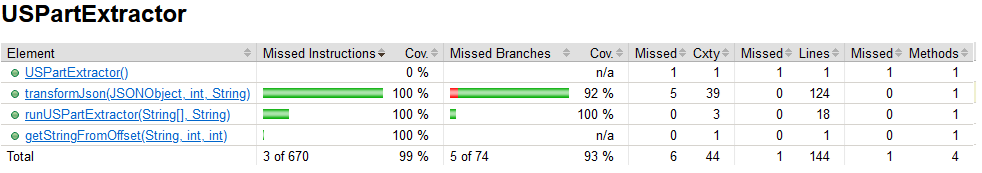
\includegraphics[scale=0.5]{code_coverage_json_transformer}
	%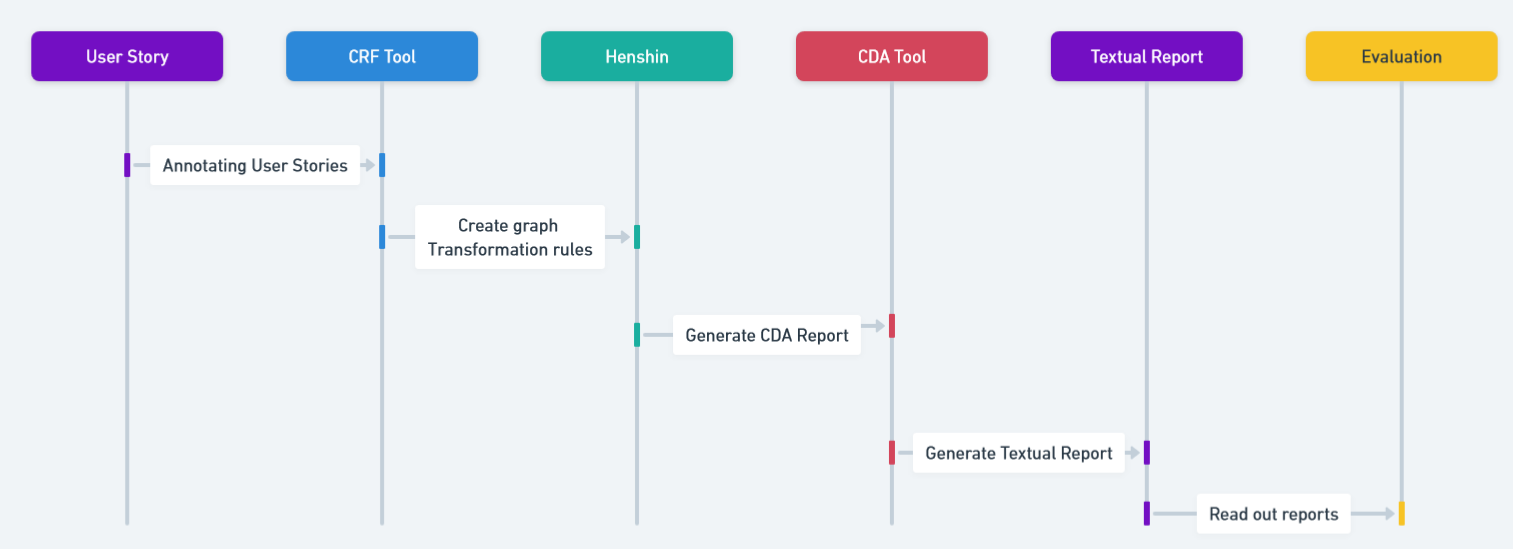
\includegraphics[scale=0.35]{sequence_diagram}
	\caption{Code coverage related to class USPartExtractor}\label{fig:code_coverage_json_transformer}
\end{figure} 


Table \ref{tb:test_cases_verb_finder} shows the test cases for the VerbFinder.java class and Figure \ref{fig:code_coverage_verb_finder} shows the code coverage.

%\end{figure}
%\end{landscape}
%\restoregeometry
%\newgeometry{margin=2.5cm}
%\begin{landscape}
	\thispagestyle{empty}
%	\begin{figure}[h]
		\begingroup
		\centering
		\scriptsize
		\renewcommand{\arraystretch}{1,5} 
		\keepXColumns
		\begin{tabularx}{\textwidth}{X  X  X  X}		
			\hline
			Test Case &Supplied Data&Expected Outcome&Description\\
			\hline\hline
			\endfirsthead
			\hline
			Test Case &Supplied Data&Expected Outcome&Description\\
			\hline\hline
			\endhead
			testLoadCSV\linebreak (Case1)&Assign a CSV file that contains two columns: one for verbs and one for action comments, so that both columns contain no empty cells&Action Annotation corresponds to verbs should be returned&Checks whether the action note has been returned accordingly in respect of the verb\\
			
			testLoadCSV\linebreak (Case2)&Assign a CSV file that contains two columns: one for verbs and one for action comments, so that one column contain empty cell&A verb without an assigned action annotation should be ignored&Checks whether the action annotation has been returned accordingly in respect of the verb\\
			\hline
				\caption{Test cases for VerbFinder class}\label{tb:test_cases_verb_finder}
		\end{tabularx}		
	%	\captionof{table}{Test cases for ReportExtractor  class}\label{tb:test_cases_report_extractor}
		\endgroup
	%\end{figure}

\begin{figure}[h]
	\centering
	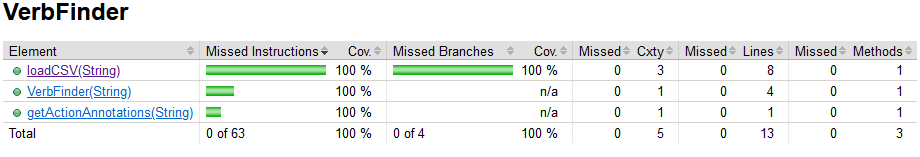
\includegraphics[scale=0.5]{code_coverage_verb_finder}
	\caption{Code coverage related to class VerbFinder}\label{fig:code_coverage_verb_finder}
\end{figure} 

Table \ref{tb:test_cases_actions_annotations_creator} shows the test cases for the ActionsAnnotationsCreator.java class and Figure \ref{fig:code_coverage_actions_annotations_creator} shows the code coverage.

%\end{figure}
%\end{landscape}
%\restoregeometry
%\newgeometry{margin=2.5cm}
%\begin{landscape}
\thispagestyle{empty}
%	\begin{figure}[h]
	\begingroup
	\centering
	\scriptsize
	\renewcommand{\arraystretch}{1,5} 
	\keepXColumns
	\begin{tabularx}{\textwidth}{X  X  X  X}		
		\hline
		Test Case &Supplied Data&Expected Outcome&Description\\
		\hline\hline
		\endfirsthead
		\hline
		Test Case &Supplied Data&Expected Outcome&Description\\
		\hline\hline
		\endhead
		ActionsAnnotationsCreator&Assign a JSON file without entries of action annotations (target or contains action annotation)&Create action annotation related to target action annotated&Checks whether the JSON array for the corresponding action has been created for the target\\
		
		
		\hline
		\caption{Test cases for ActionsAnnotationsCreator class}\label{tb:test_cases_actions_annotations_creator}
	\end{tabularx}		
	%	\captionof{table}{Test cases for ReportExtractor  class}\label{tb:test_cases_report_extractor}
	\endgroup
	%\end{figure}
	
	\begin{figure}[h]
		\centering
		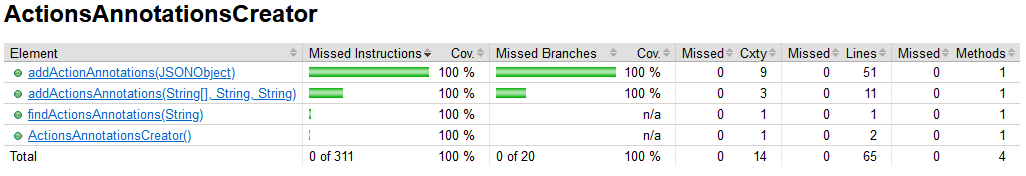
\includegraphics[scale=0.5]{code_coverage_actions_annotations_creator}
		\caption{Code coverage related to class ActionsAnnotationsCreator}\label{fig:code_coverage_actions_annotations_creator}
	\end{figure} 
	
Table \ref{tb:test_cases_report_maker} shows the test cases for the Evaluation.java class and Figure \ref{fig:code_coverage_report_maker} shows the code coverage.

%\newgeometry{margin=2.5cm}
%\begin{landscape}
%\thispagestyle{empty}
%\begin{figure}[h]
\begingroup
\centering
\scriptsize
\renewcommand{\arraystretch}{1,5} 
\keepXColumns

\begin{tabularx}{\textwidth}{X  X  X  X}
	\hline
	Test Case &Supplied Data&Expected Outcome&Description\\
	\hline\hline
	\endfirsthead
	\hline
	Test Case &Supplied Data&Expected Outcome&Description\\
	\hline\hline
	\endhead
	
	ActionAnnotation\newline InJsonFileNotFound&Provision of a JSON object without action annotation&Through an exception:\textit{ActionAnnotation InJsonFileNotFound}&Checks whether the JSON object provided contains an entry for action annotations\\
	
	TargetActionAnnotation\newline InJsonFileNotFound&Provision of a JSON object without target action annotation&Through an exception:\textit{ActionAnnotation InJsonFileNotFound}&Checks whether the JSON object provided has an entry for target action annotations\\
	
	ContainActionAnnotation\newline InJsonFileNotFound&Provision of a JSON object without contain action annotation&Through an exception:\textit{ActionAnnotation InJsonFileNotFound}&Checks whether the JSON object provided has an entry for contain action annotations\\
	
	EntityContainExist&Provision of a conflict pair with indirect conflict through contain relation&The US-pairs should be reported as a conflict pair&Checks whether the conflict is recognised if the entity from Us belongs to contain relation\\
	
	JsonArrayNotFound&Provision of a JSON file in which a JSON array is missing&Null should be return&Checks whether the specific JSON array was not found, if so, return null\\
	
	JsonObjectNotFound&Provision of a JSON file in which a JSON object is missing&Null should be return&Checks whether the specific JSON object was not found, if so, return null\\
	
	runReportMaker\_Main&Provision of two USs that contradict each other&The conflict pair should be reported in text form&Checks whether two USs that contradict each other have already been reported as conflict pair\\
	
	MainIsEmpty&Provision of a JSON object with empty main part entry&Through an exception:\textit{MainPartInJsonFile NotFound }&Checks whether the main part entry in provided JSON object is not empty\\
	
	MainNotExist&Provision of a JSON object without main part entry&Through an exception:\textit{MainPartInJsonFile NotFound }&Checks whether the JSON object provided has main part entry\\
	
	runReportMaker\_NoConflict&Provision of a set of USs that not contradict each other&The conflict pair should not be reported&Checks whether two USs that do not contradict each other should not be reported as a conflict pair\\
	
	UsNrInJsonFileNotFound&Provision of a JSON object that don't have US identifier&Through an exception:\textit{UsNrInJsonFileNotFound}&Checks whether the JSON object in the JSON file already has an identifier\\
	
	writeTable&Provision of a conflict pair that should be reported&Conflict pair should be listed in tabular form&Check whether the conflict pair is already listed in the table\\
	\hline
	\caption{Test cases for ReportMaker  class}\label{tb:test_cases_report_maker}
\end{tabularx}

%\captionof{table}{Test cases for RuleCreator  class}\label{tb:test_cases_rule_creator}
\endgroup
\thispagestyle{empty}
%\end{landscape}
%\restoregeometry

\begin{figure}[h]
	\centering
	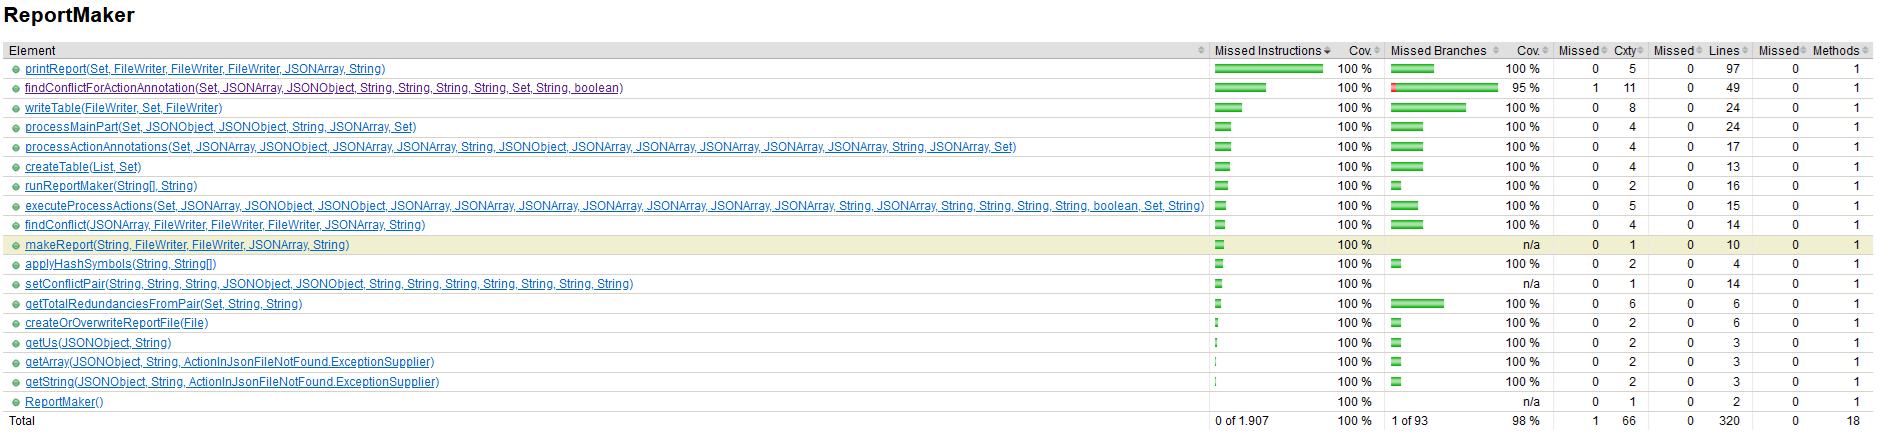
\includegraphics[scale=0.3]{code_coverage_report_maker}
	%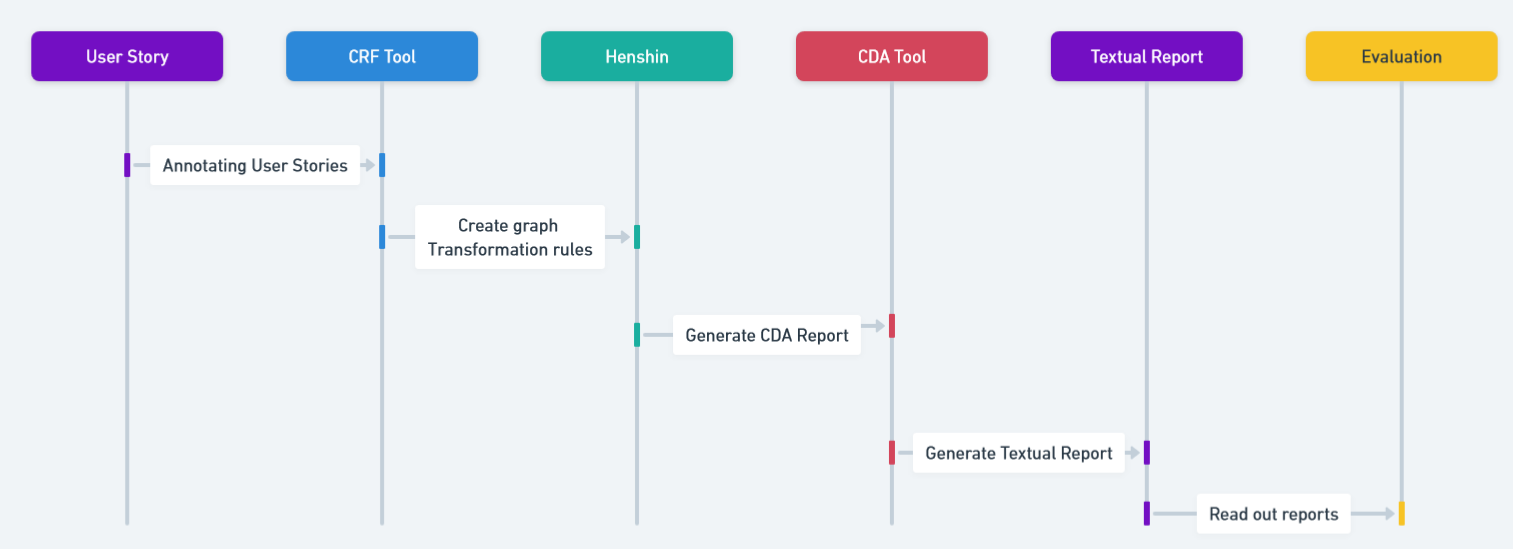
\includegraphics[scale=0.35]{sequence_diagram}
	\caption{Code coverage related to class ReportMaker}\label{fig:code_coverage_report_maker}
\end{figure}
%\subsubsection*{Performance Test}
%In this section, we describe the performance testing approach used for this project, including the test setup, key metrics, and the results of the tests.

\subsection{Evaluation}\label{conflict_evaluation}
In this section, we address two research questions (RQs) and explain how we designed and conducted the experiments for each question. We then analyse the results to answer these RQs, discuss their significance and share the findings from the results.
\subsubsection*{Research Questions}
The RQs addressed in this section are as follows:
\begin{itemize}
	\item \textbf{RQ 1}: Does our tool consistently identify conflicts between USs?
	\item \textbf{RQ 2}: How does the performance of the tool change as the count of USs in a backlog increases?
	\end{itemize}
\subsubsection*{Methodology}
To answer the RQ1, "Does our tool consistently detect conflicts between USs?", we recapitulate the methodology used to analyse conflicts between USs. We used a systematic approach that includes several important steps:
\begin{itemize}
	
	\item Data Collection: For a comprehensive assessment, we applied our approach to 19 backlog datasets presented by Mosser et al. \footnote{\href{https://github.com/ace-design/nlp-stories}{https://github.com/ace-design/nlp-stories}}. They applied the Doccano approach to these publicly available requirements datasets \cite{requirementsdatasets}.
	
	 It is also worth noting that some backlog datasets (g02, g13, g17, g27) did not follow the expected sentence structure, so we did not include them in the evaluation results to avoid unexpected behaviour. Table \ref{tb:conflcit_backlogs} shows the project number of each dataset and the count of USs.
	 
	 %empty line here
	\begingroup
	\centering
	\scriptsize
	\renewcommand{\arraystretch}{1.5} 
	\begin{tabularx}{\linewidth}{l|XXXXXXXXXXXXXXXXXXX X}
		Item&	1&	2&	3&	4&	5&	6&	7&	8&	9&	10&	11&	12&	13&	14&	15&	16&	17&	18&	19&	\\
		\hline
		Project Nr.&	g03	&g04	&g05	&g08	&g10	&g11	&g12	&g14	&g16	&g18	&g19	&g21	&g22	&g23	&g24	&g25	&g26	&g27	&g28	&Total USs\\
		\hline
		Total USs&	57&	51	&53	&66	&97	&73	&54	&67	&66	&102	&137	&69	&83	&56	&53	&100	&100	&114	&60	&1458 \\
		\caption{Project number and count of USs contained in each backlog dataset}\label{tb:conflcit_backlogs}
	\end{tabularx}	
	\endgroup
	\item Splitting the elements of the US into main and benefit parts: each element of the US (action, entity and relations) was split into main or benefit part, where the main part represents the core functionality and the benefit part describes the value for the persona. In this analysis, we only consider the conflicts between the main parts of the USs.
	
	\item Recognition of conflicts: Detection of conflicts between USs in main parts of the USs based on defined criteria.
	
\end{itemize}
\subsubsection*{Ground Truth}
To answer the first research question (RQ), our automated system needs a reference point to measure its accuracy. This reference point, called "ground truth", comes from a personal judgement and serves as a benchmark for evaluating the tool's performance.

Unlike the tool evaluation, we did not assess conflicts based on defined criteria. Instead, in the ground truth evaluation, we examined conflicts based on the text of the US-pairs detected by tool. This involved reading the text of the USs and evaluating conflicts between US-pairs in a semantic manner.

The ground truth serves as the final assessment against which the automated results are compared. It results from the personal judgement of a subject matter expert (in this case me) using a combination of expertise and experience. This personal judgement is intended to provide a reliable and accurate reference for identifying conflicts between USs.\\\\
Table \ref{tb:conflict_ground_truth} shows the summary of conflicting US-pairs as ground truth.
\begin{figure}[h]
	\begingroup
	\scriptsize
	\centering
	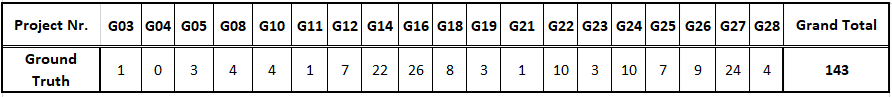
\includegraphics[scale=0.6]{Table/conflict_ground_truth.png}
	\captionof{table}{Details of the count of correctly recognised and validated conflicting US-pairs by the tool as ground truth}\label{tb:conflict_ground_truth}	
	\endgroup
\end{figure}
\subsubsection*{Evaluating Tool-Detected Conflicts Using Ground Truth}
The automated tool was developed to recognise conflicts between USs based on predefined criteria. It analyses the structure of USs to identify discrepancies that could indicate a conflict.

In contrast to ground truth, which is based on the semantic comparison of texts in the main parts of USs, the evaluation of the tool relies heavily on specified labelling (targets, triggers, contains) using the Doccano tool and predefined criteria.

Table \ref{tb:tool} shows the aggregation of the conflicting US-pairs found in the main parts evaluated by the tool.
\begin{figure}[h]
	\begingroup
	\scriptsize
	\centering
	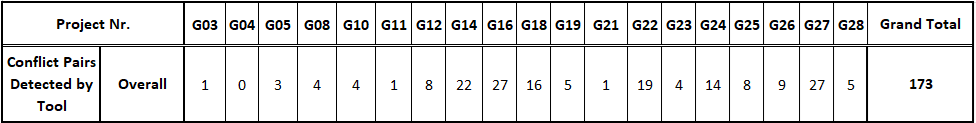
\includegraphics[scale=0.55]{Table/conflict_tool.png}
	\captionof{table}{Overall count of conflicting US-pairs in relation to the main parts assessed by the tool}\label{tb:conflict_tool}
	\endgroup
\end{figure}
\paragraph{Assessment of Result: High-Level Overview}When comparing the results provided by the tools with the ground truth, we found that 143 cases were correctly assessed as conflicting US-pairs and 30 cases were invalid on the basis of the ground truth.

Table \ref{tb:conflict_difference} shows the count of valid and invalid conflicting US-pairs assessed by the ground truth and recognised by the tool.

Based on the datasets provided, 173 conflicting US-pairs were found across all projects, with the highest count found in the backlog G27 dataset (24 cases), indicating a significant occurrence of conflicts in the USs of this project.
\begin{figure}[h]
	\begingroup
	\scriptsize
	\centering
	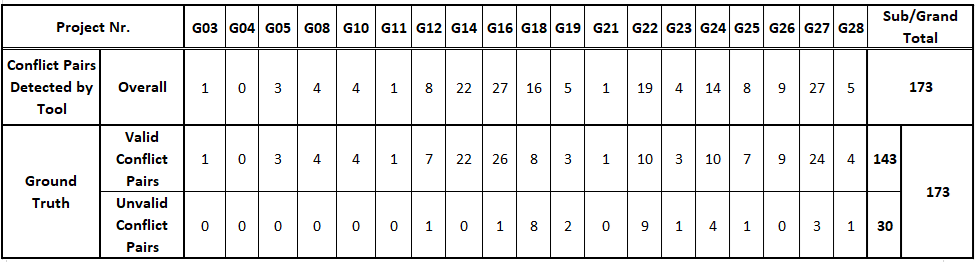
\includegraphics[scale=0.55]{Table/conflict_difference.png}
	\captionof{table}{Information on the number of discrepancies between the result provided by the tool and the ground truth}\label{tb:conflict_difference}
	
	\endgroup
\end{figure}
\paragraph{Assessment of Result: Detailed Insights}In the USs of the datasets, there are some verbs such as "have", "know" and nouns such as "data", "resource", "collection", "list", and "file" that are cross-contextual, so they do not contain generic information, which has a very negative impact on conflicts analysis (30 cases are false positives).

\begin{example}
	For example, user\_story\_983 and user\_story\_989 are reported as a conflicting US-pair in the G24 backlog dataset:\\
	\textit{user\_story\_1365:} \#G24\# As a depositor, I want to store and manage \#datasets\# via a simple web interface.\\
	\textit{user\_story\_1409:} \#G24\# As a research information manager, I want to have \#datasets\# linked to metadata about projects.\\
	The depositor needs a simple interface for uploading and managing datasets. The research information manager needs to be able to link these datasets to comprehensive metadata about the projects.\\
	These needs are not inherently conflicting, but they require careful design consideration to ensure that both needs are met effectively.\\
	To avoid the conflict, the verb "have" related to "user\_story\_1409" should be defined more precisely. The US should be amended as follows:\\
	\textit{user\_story\_1409:} \#G24\# As research information manager, I want to \textit{\texttt{link} \texttt{datasets}} to metadata about projects.\\
\end{example}

There are also annotated USs with inaccurate labelling by the Doccano tool. In other words, there is more information about the resource in concern provided in US, which leads to inconsistencies and bias.
\begin{example}
	In the dadaset of backlog G25, for example, we have a US-pair that are marked as conflict:\\
	\textit{user\_story\_1506}: \enquote{\#G25\# As a DAMS manager, I want to know when the \#application\# of a statute to an object or object component has been \#modified\#, either manually or automatically.}\\
	\textit{user\_story\_1510:} \enquote{\#G25\# As a DAMS manager, I want to know if \#application\# of a library policy to an object or object component has been \#modified\#, either manually or automatically.}\\
	In the annotated dataset, the identified entities of "user\_story\_1506" and "user\_story\_1510" are only \enquote{application}, which is not fully labelled. The correct labelling for "user\_story\_1506" should be \texttt{"application of a statute"} and for "user\_story\_1510" should be \texttt{"application of a library policy"}. With these changes, no conflict will be reported between these two USs.
\end{example}
\paragraph{RQ1: Conclusion}
After comparing the ground truth result with the result provided by our tool, we find that 83\% of the conflicting US-pairs found are valid and only 17\% of the cases are invalid which is classically considered as excellent.

The results of the automated tool are consistent with the ground truth, which shows that it reliably recognises conflicts. This agreement with personal judgements increases confidence in the accuracy and validity of the tool. 

The tool also demonstrates its effectiveness and trustworthiness. This reliability means that users can rely on the tool to accurately identify conflicts, reducing the need for extensive manual review. 
\subsubsection*{Performance Evaluation}
To answer the RQ2 "How does the performance of the tool change as the count of USs in a backlog increases?", we conducted a series of tests to measure the time it takes the tool to process different counts of USs. This section describes the test method, the results obtained and the impact on the scalability of the tool.
\paragraph{Test Methodology}To evaluate the tool's performance, we conducted a set of experiments in which the tool processed different numbers of USs in a backlog. The tests involved the following steps:
\begin{enumerate}
	\item Backlog Setup: We used backlogs with varying numbers of USs around—50, 70, 90, 120 and 140—to simulate different workload sizes. Each backlog contained USs with varying content, and complexity to represent a realistic range of cases. Table \ref{tb:conflict_performance_env} shows information on the backlog data records provided for the performance test application.
	\begin{figure}[h]
		\begingroup
		\scriptsize
		\centering
		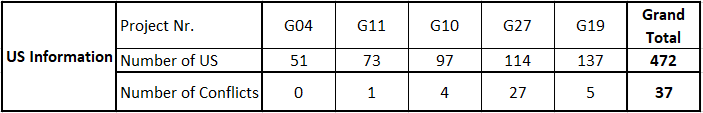
\includegraphics[scale=0.7]{Table/conflict_performance_env.png}
		\captionof{table}{Information on the backlog datasets provided for the application of the performance test}\label{tb:conflict_performance_env}
		\endgroup
	\end{figure}
	\item Tool Execution: Each part of toolchain (USPartExtractor, ActionsAnnotationsCreator, and ReportMaker) was run for each backlog and the total time taken to process the entire backlog was recorded. The performance of the tool was measured by the processing time, i.e. the total time taken to process all USs in the backlog and identify conflicts and reporting.
	
	\item Repeating Tests: To ensure reliability, each test was conducted multiple times, and the average processing time was calculated.
\end{enumerate}
The test environment consisted of:
\begin{itemize}
	\item Processor: Intel(R) Core(TM) i7-8565U CPU @ 1.80GHz (8 CPUs), ~2.0GHz		
	\item Memory: 8070MB RAM
	\item Display Devices: Intel(R) UHD Graphics 620, 4163 MB(Display Memory)
	\item Hard Disk: INTEL SSDPEKNW512G8H
	\item Operating System: Windows 11 Home 64-bit (10.0, Build 22631) (22621.ni\_release .220506-1250)
	\item System Type: 64-bit operating system, x64-based processor
\end{itemize}
Table \ref{tb:conflict_performance_result} shows the result of tool's performance in seconds which were conducted on a controlled environment to ensure consistency.
	\begin{figure}[h]
	\begingroup
	\scriptsize
	\centering
	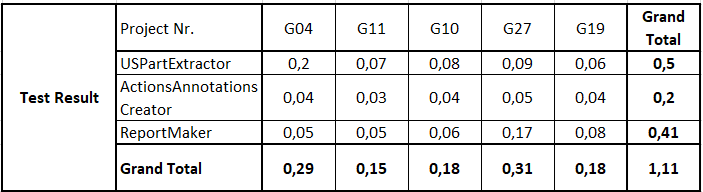
\includegraphics[scale=0.75]{Table/conflict_performance_result.png}
	\captionof{table}{Information about the result of the tool's performance test, which was measured using the processing time in seconds.}\label{tb:conflict_performance_result}
	\endgroup
\end{figure}
\paragraph{RQ2: Conclusion}There is no direct relationship between the count of USs in a backlog and the processing time required by our tool (G27 vs G19).
However, there is a direct relationship between the count of conflicts found between USs and the processing time. The more conflicts there are, the longer the processing time. 

Overall, developers and project managers with a growing backlog can expect the tool to take a reasonable amount of time to assess conflicts.
\subsubsection*{Threats to Validity}
Several potential threats to validity need to be considered when assessing the conflicts between USs both by personal judgement (ground truth) and by the automated tool. This section outlines the main threats to validity and describes how they were mitigated during the study.
\paragraph{Construct validity}It refers to how accurately the assessment measures what it is supposed to measure. The following risks have been identified:
\begin{itemize}
	\item Ambiguity of criteria: If the criteria for conflict are unclear or open to interpretation, this can lead to inconsistent scores. To avoid this, we defined clear and detailed criteria for identifying conflicts in USs.
	
	\item Ambiguity of action-annotations: If the action-annotations associated with each verb in a US are unclear or not specific to the context, this can lead to inconsistent scores. To prevent this, we assign the action-annotations based on the context of the backlog instead of using general terms.
	
	\item Subjectivity in ground truth: Since the ground truth is based on personal judgements, subjectivity could lead to bias. To minimise this risk, the evaluator (in this case me) has cross-checked the evaluations several times.
\end{itemize}
\paragraph{External validity}External validity refers to how well the results of the study can be transferred to other contexts or populations. Threats to external validity include:

\begin{itemize}
	\item specificity of USs: If the USs in the study are too specific or specific to the context, the results may not be transferable to other projects. To avoid this, we analysed 19 backlog datasets with different USs and project types.
	
	\item Tool Limitations:
	\begin{itemize}
		
	 \item The automated tool is tailored to a specific format of USs, which limits its wider applicability. It is highly dependent on the exact structure of USs (e.g. "As \textless role\textgreater I want to ..., so that ..."), which is crucial for its functionality. Therefore, we evaluated the tool in controlled environments, focussing exclusively on well-structured USs, and investigated its performance in different scenarios.
	
	\item Our tool relies on a specific type of annotations for USs, e.g. action, entity, their reference targets, triggers and contains. The effectiveness of the tool depends on these annotations being accurate and consistent. If the annotations are incomplete or incorrect, the tool may not work properly. Also, the tool may not be compatible with other annotation schemes that use different labels.
	
	\item The verbs in the action-annotation reference database are not included in their root form, but as they actually occur in the USs. This means that the same verb in different forms may be found in the database.
\end{itemize}
\end{itemize}
\paragraph{Internal Validity}Internal validity is concerned with whether the observed results are attributable to the factors analysed or are influenced by other variables. Potential threats to internal validity include:
\begin{itemize}
	\item Confounding factors: External factors or unintended variables can influence the evaluation of the conflicts analysis. In particular, the USs annotated with Doccano have a significant influence on the conflicts analysis. The more phrases are covered as label (especially as entity and action), the better the result of evaluation. Since our tool uses Doccano-annotated USs without changes as primary input, these discrepancies are unavoidable.
	
	\item Limitation of tool: The automated tool does not take into account the analysis of conflicts in the benefit parts of the USs.
\end{itemize}
\subsection{Conclusion}\label{conflict_conclustion}
In this study, we introduced an approach that integrates the Doccano tool and our custom tool to systematically identify and report conflicts between USs in software development projects. We also conducted an evaluation of this approach.

By carefully analysing 19 different backlog datasets, our method not only separated the USs into main and benefit parts for nuanced examination, but also facilitated conflicts analysis by translating the verbs of the main parts into four distinct categories, namely "delete", "create", "forbid" and "preserve", and finally reported the potential conflicts in text base format.

Our results reveal a decisive finding: the effectiveness of conflicts analysis is significantly influenced by the quality of the USs and their annotations. Well-formulated USs, in which general verbs (e.g. "have", "know") and nouns (e.g. "data", "list", "collection") are avoided, as well as a concisely annotated backlog with precise labelling of the entities (nouns) significantly improve the effectiveness of the conflicts analysis.

 If the main parts of a US-pair contradict each other, the application of one US has a negative effect on another US by deleting a resource that another US uses, or creating a resource that another US prohibits, or deleting a resource that another US also wants to delete.
 
 If conflicts between USs are identified, this is a signal for the project team to take a closer look at the requirements and the design of the system. By prioritising, sequencing, defining clear rules, implementing conflict resolution mechanisms, refining USs and involving stakeholders, the team can effectively manage and resolve these conflicts to ensure a well-functioning system.
 
In summary, our study confirms the central role of a semantic analysis approach in the detection and management of conflicts in project backlogs and thus contributes to the rationalisation of software development processes.

The quality of the annotated USs and their well-formed structure are central to the success of this approach. The results of this study provide useful guidance for improving current practices and shaping future research in software project management.

